\section{Результаты}

\begin{figure}[H]
	\begin{tabular}{ccc}
		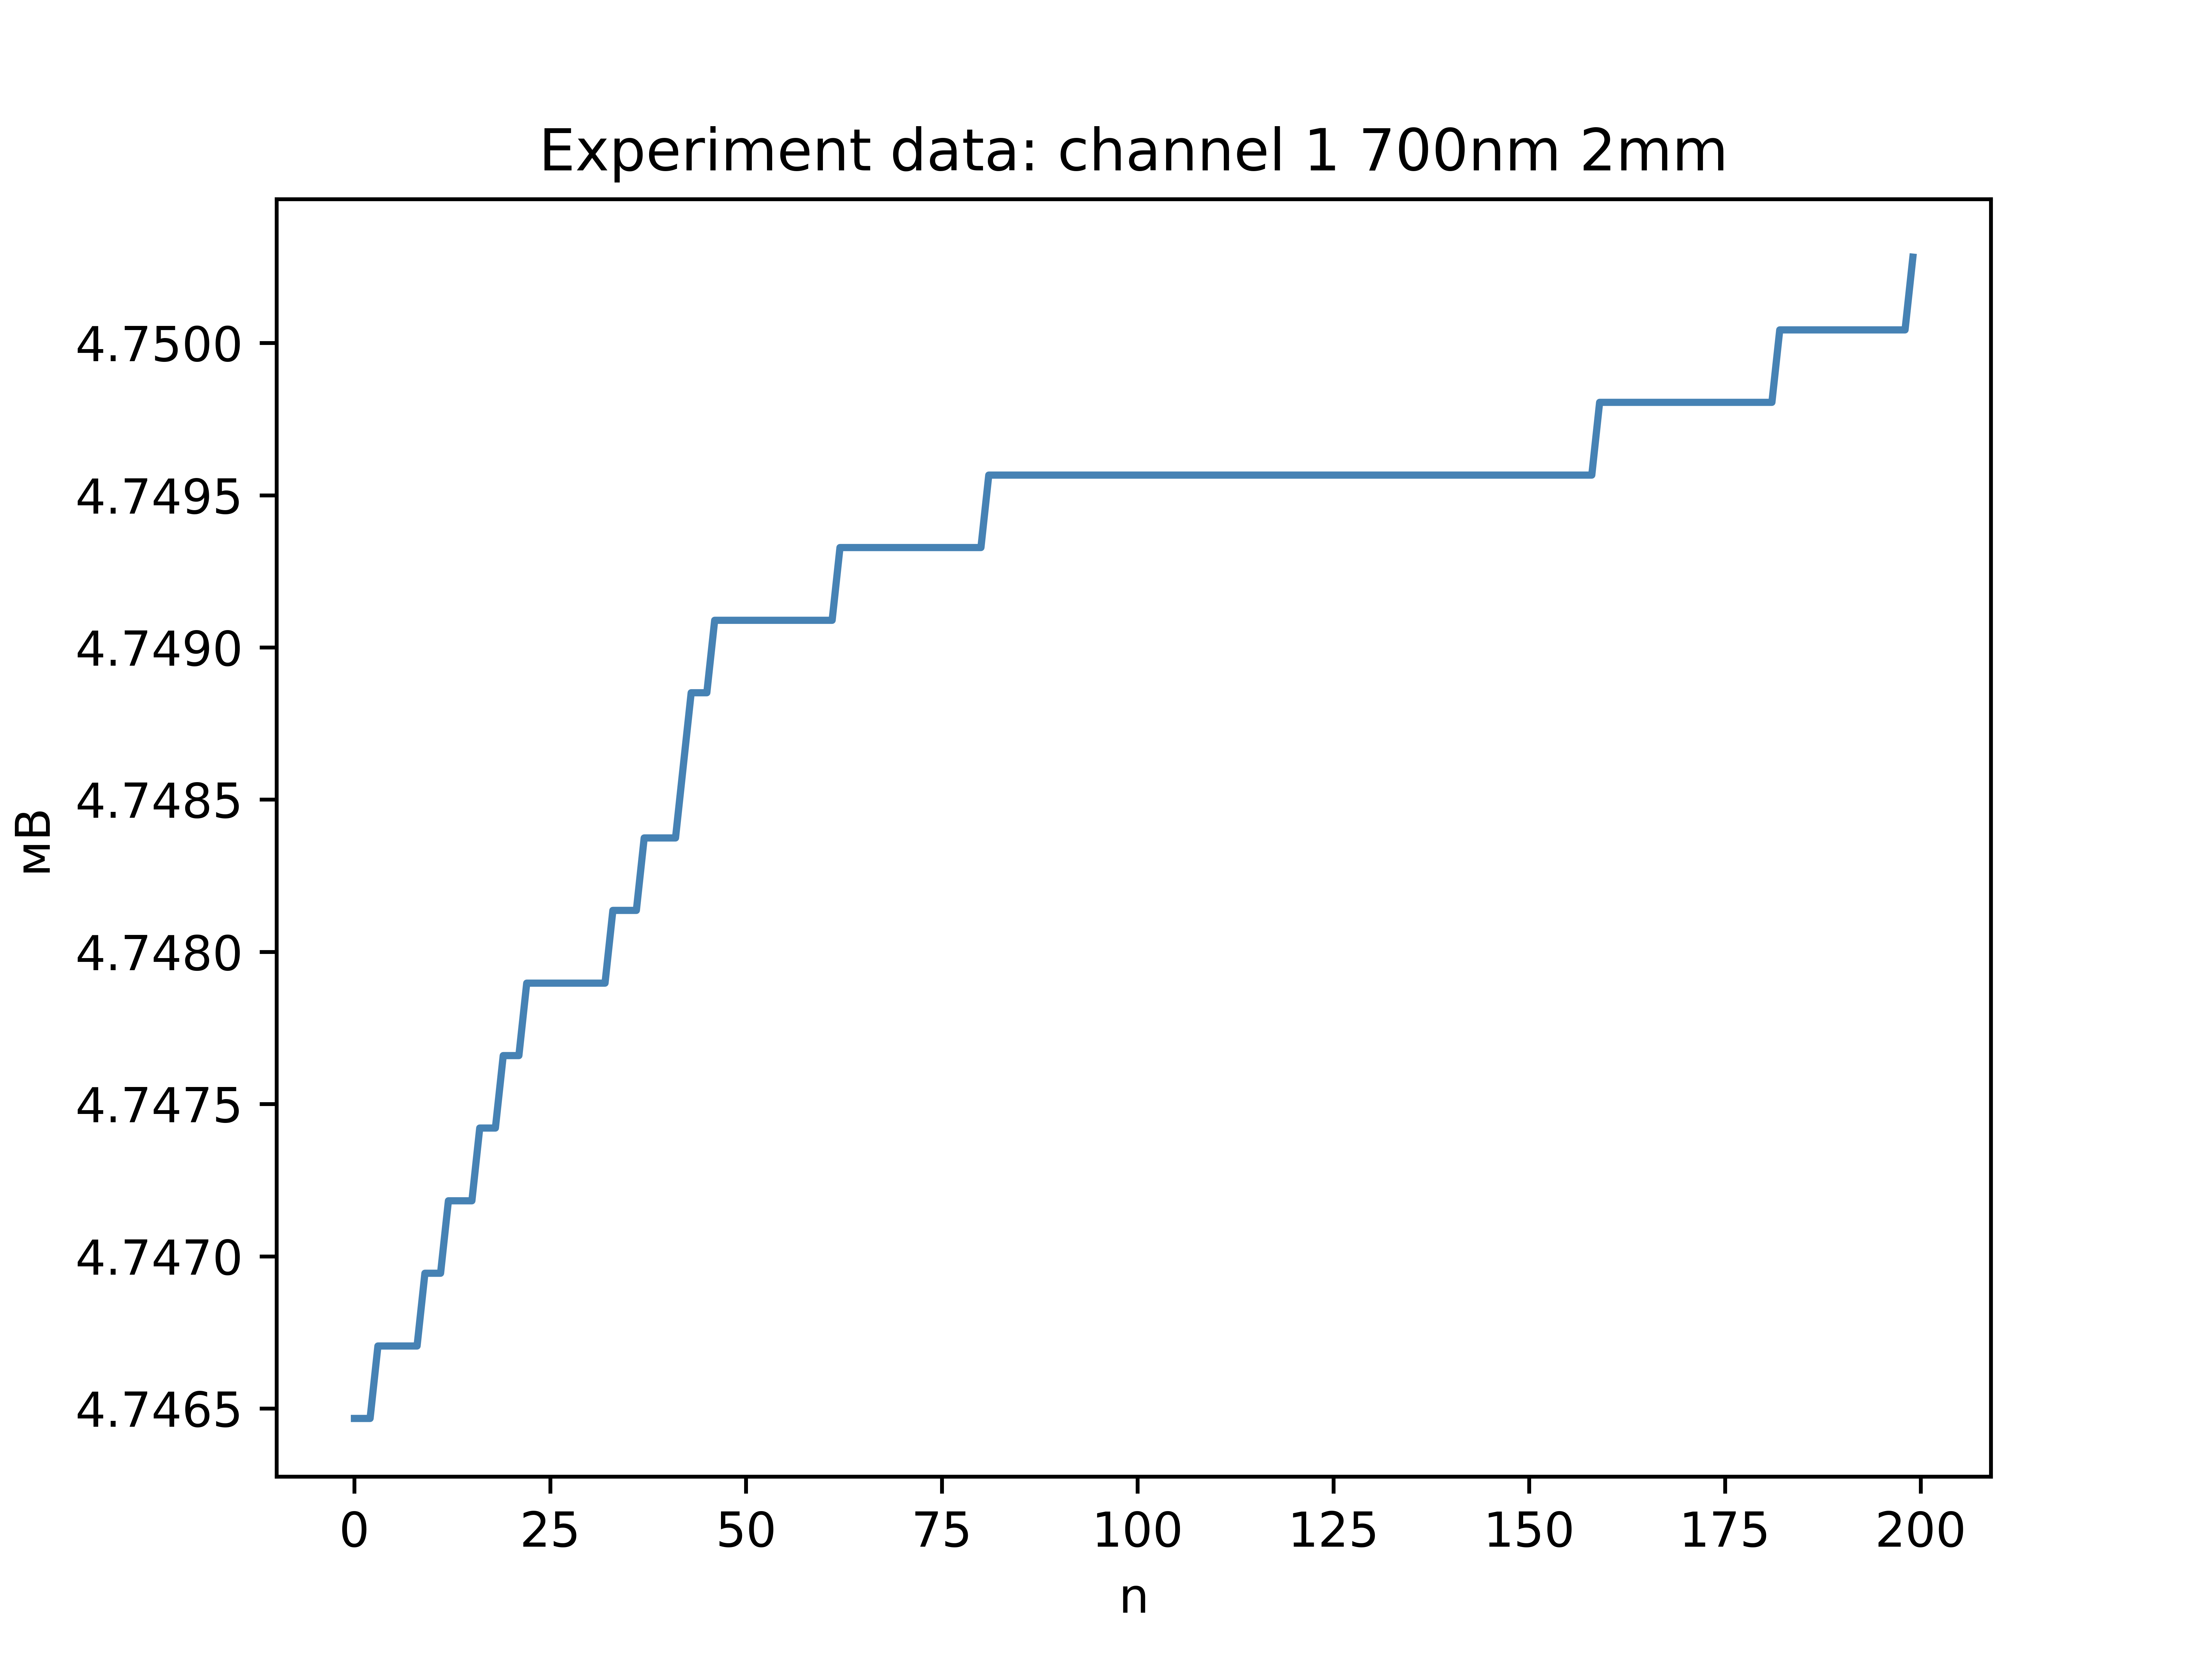
\includegraphics[scale=0.5]{resources/input_PR1.png}
		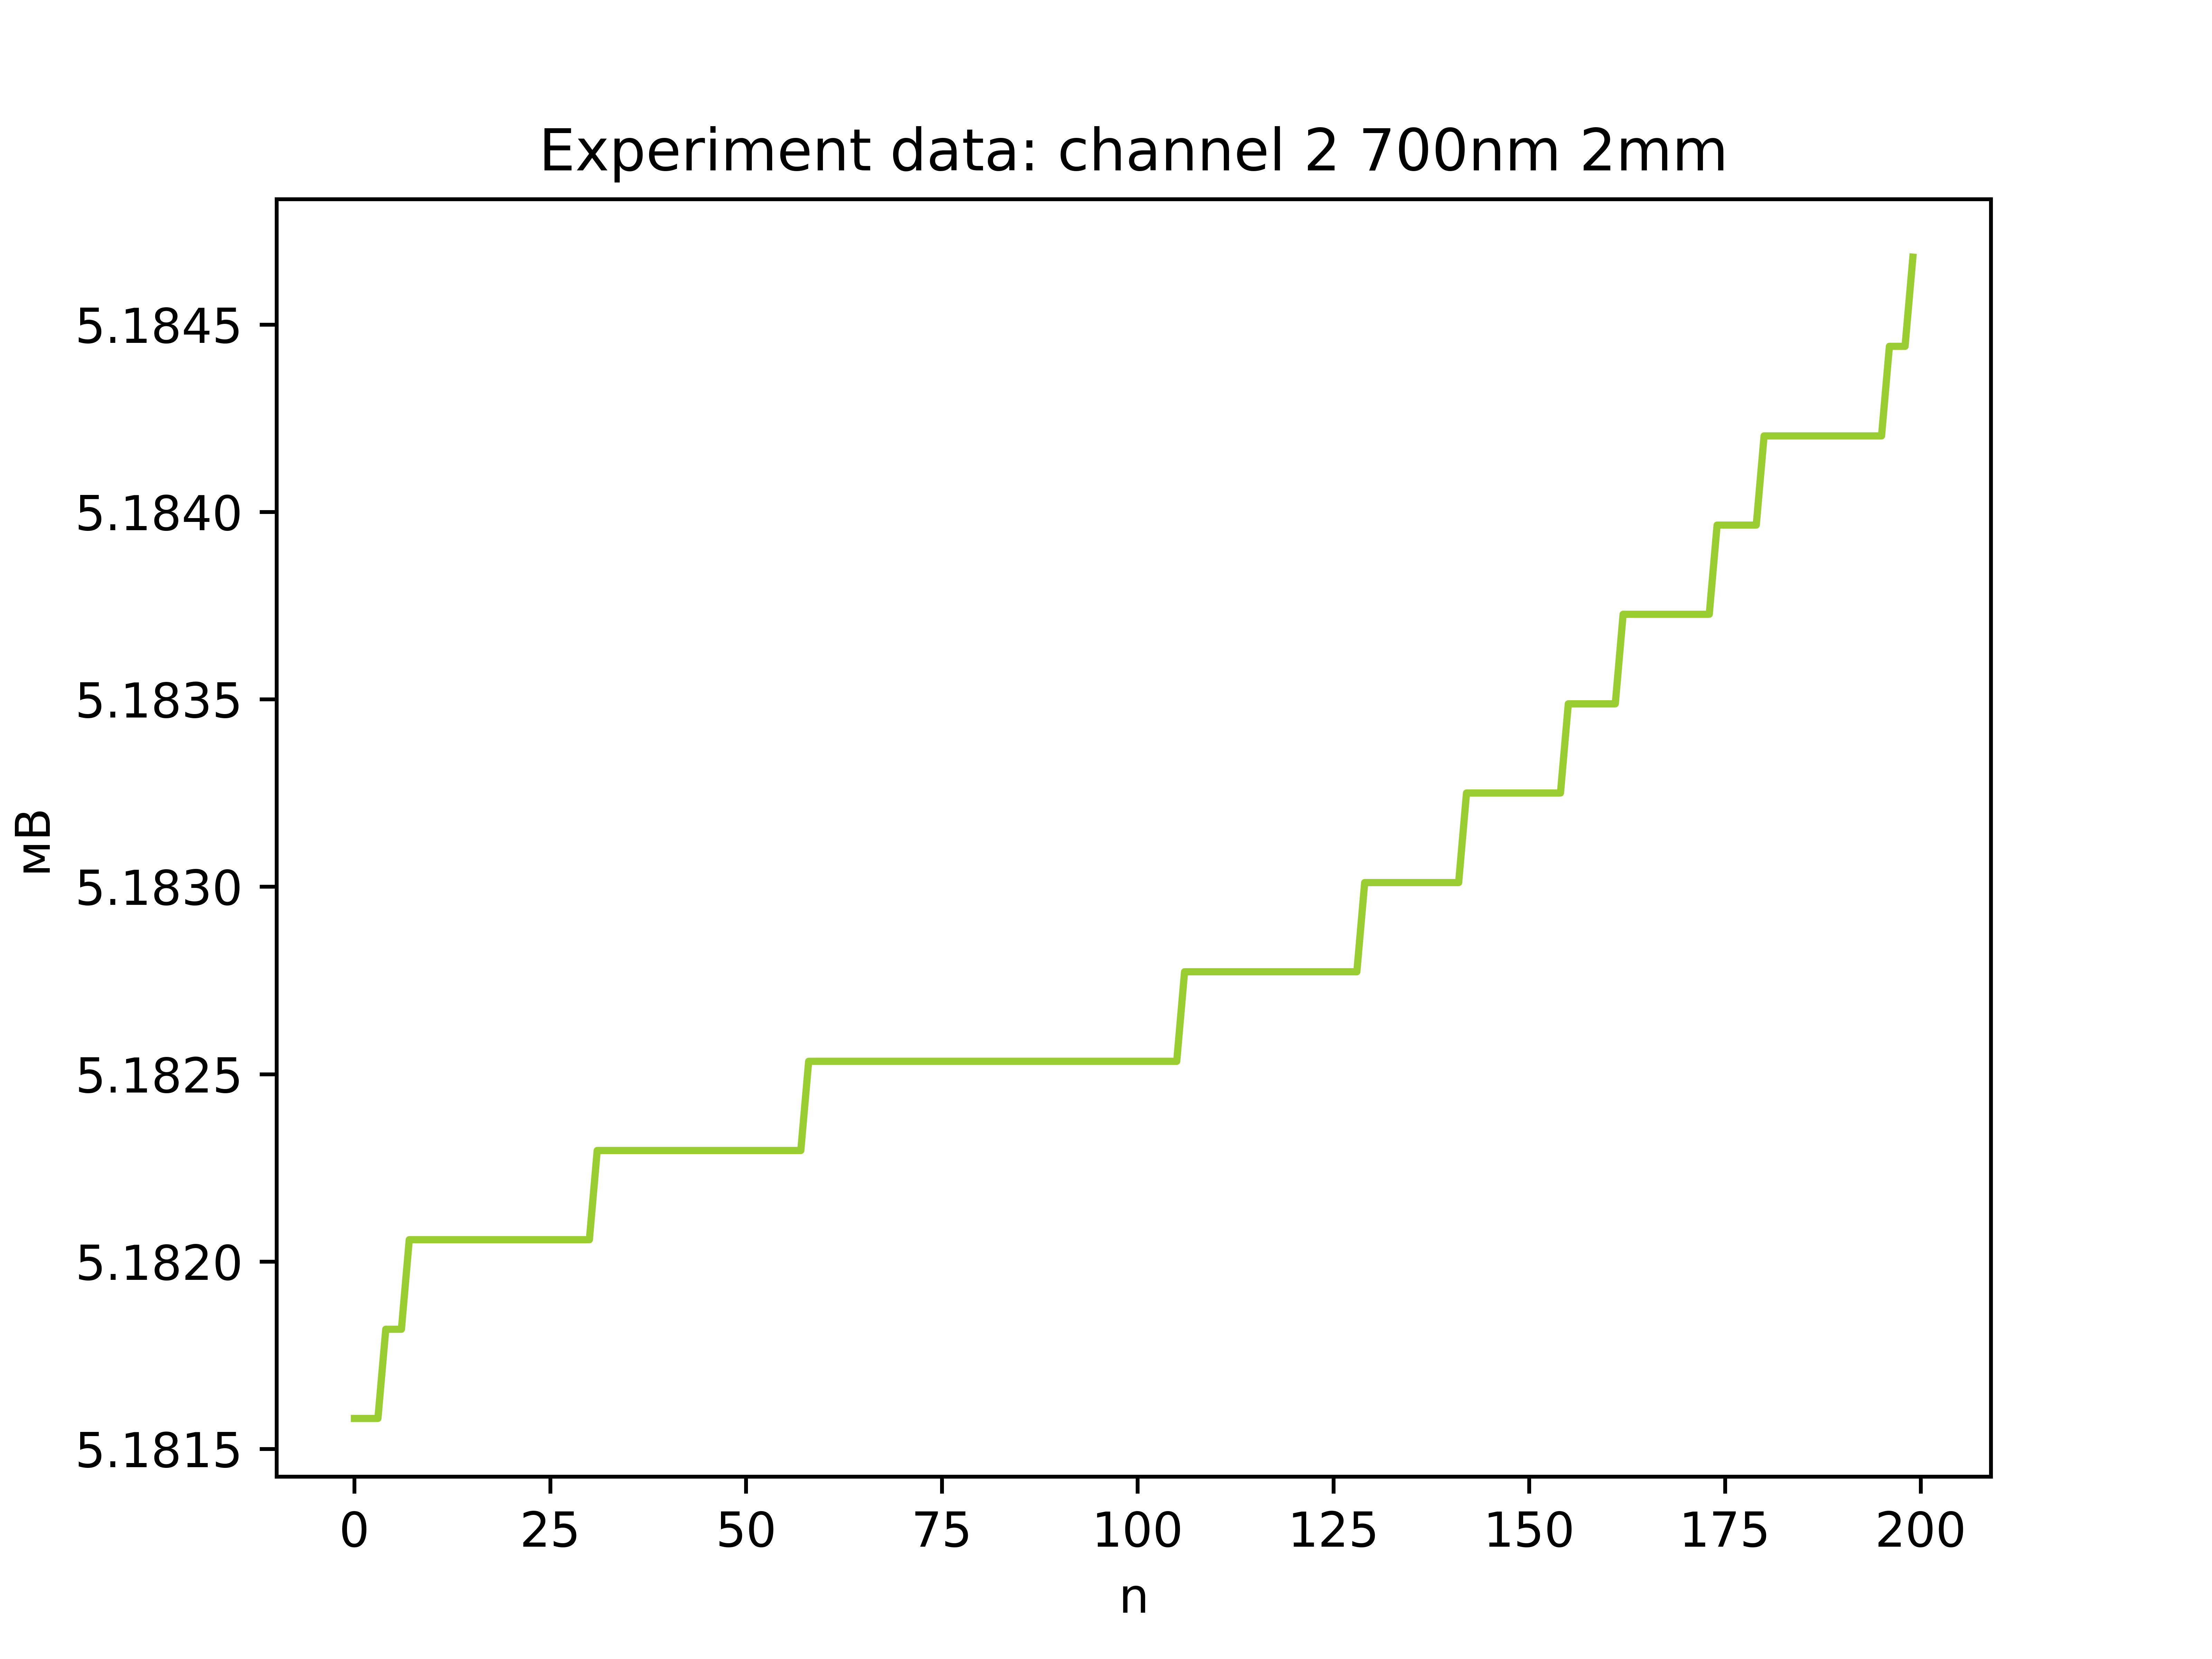
\includegraphics[scale=0.5]{resources/input_PR2.png}
	\end{tabular}
	\caption{Исходные данные из экспериментов} 
\end{figure}

\begin{figure}[H]
	\begin{tabular}{ccc}
		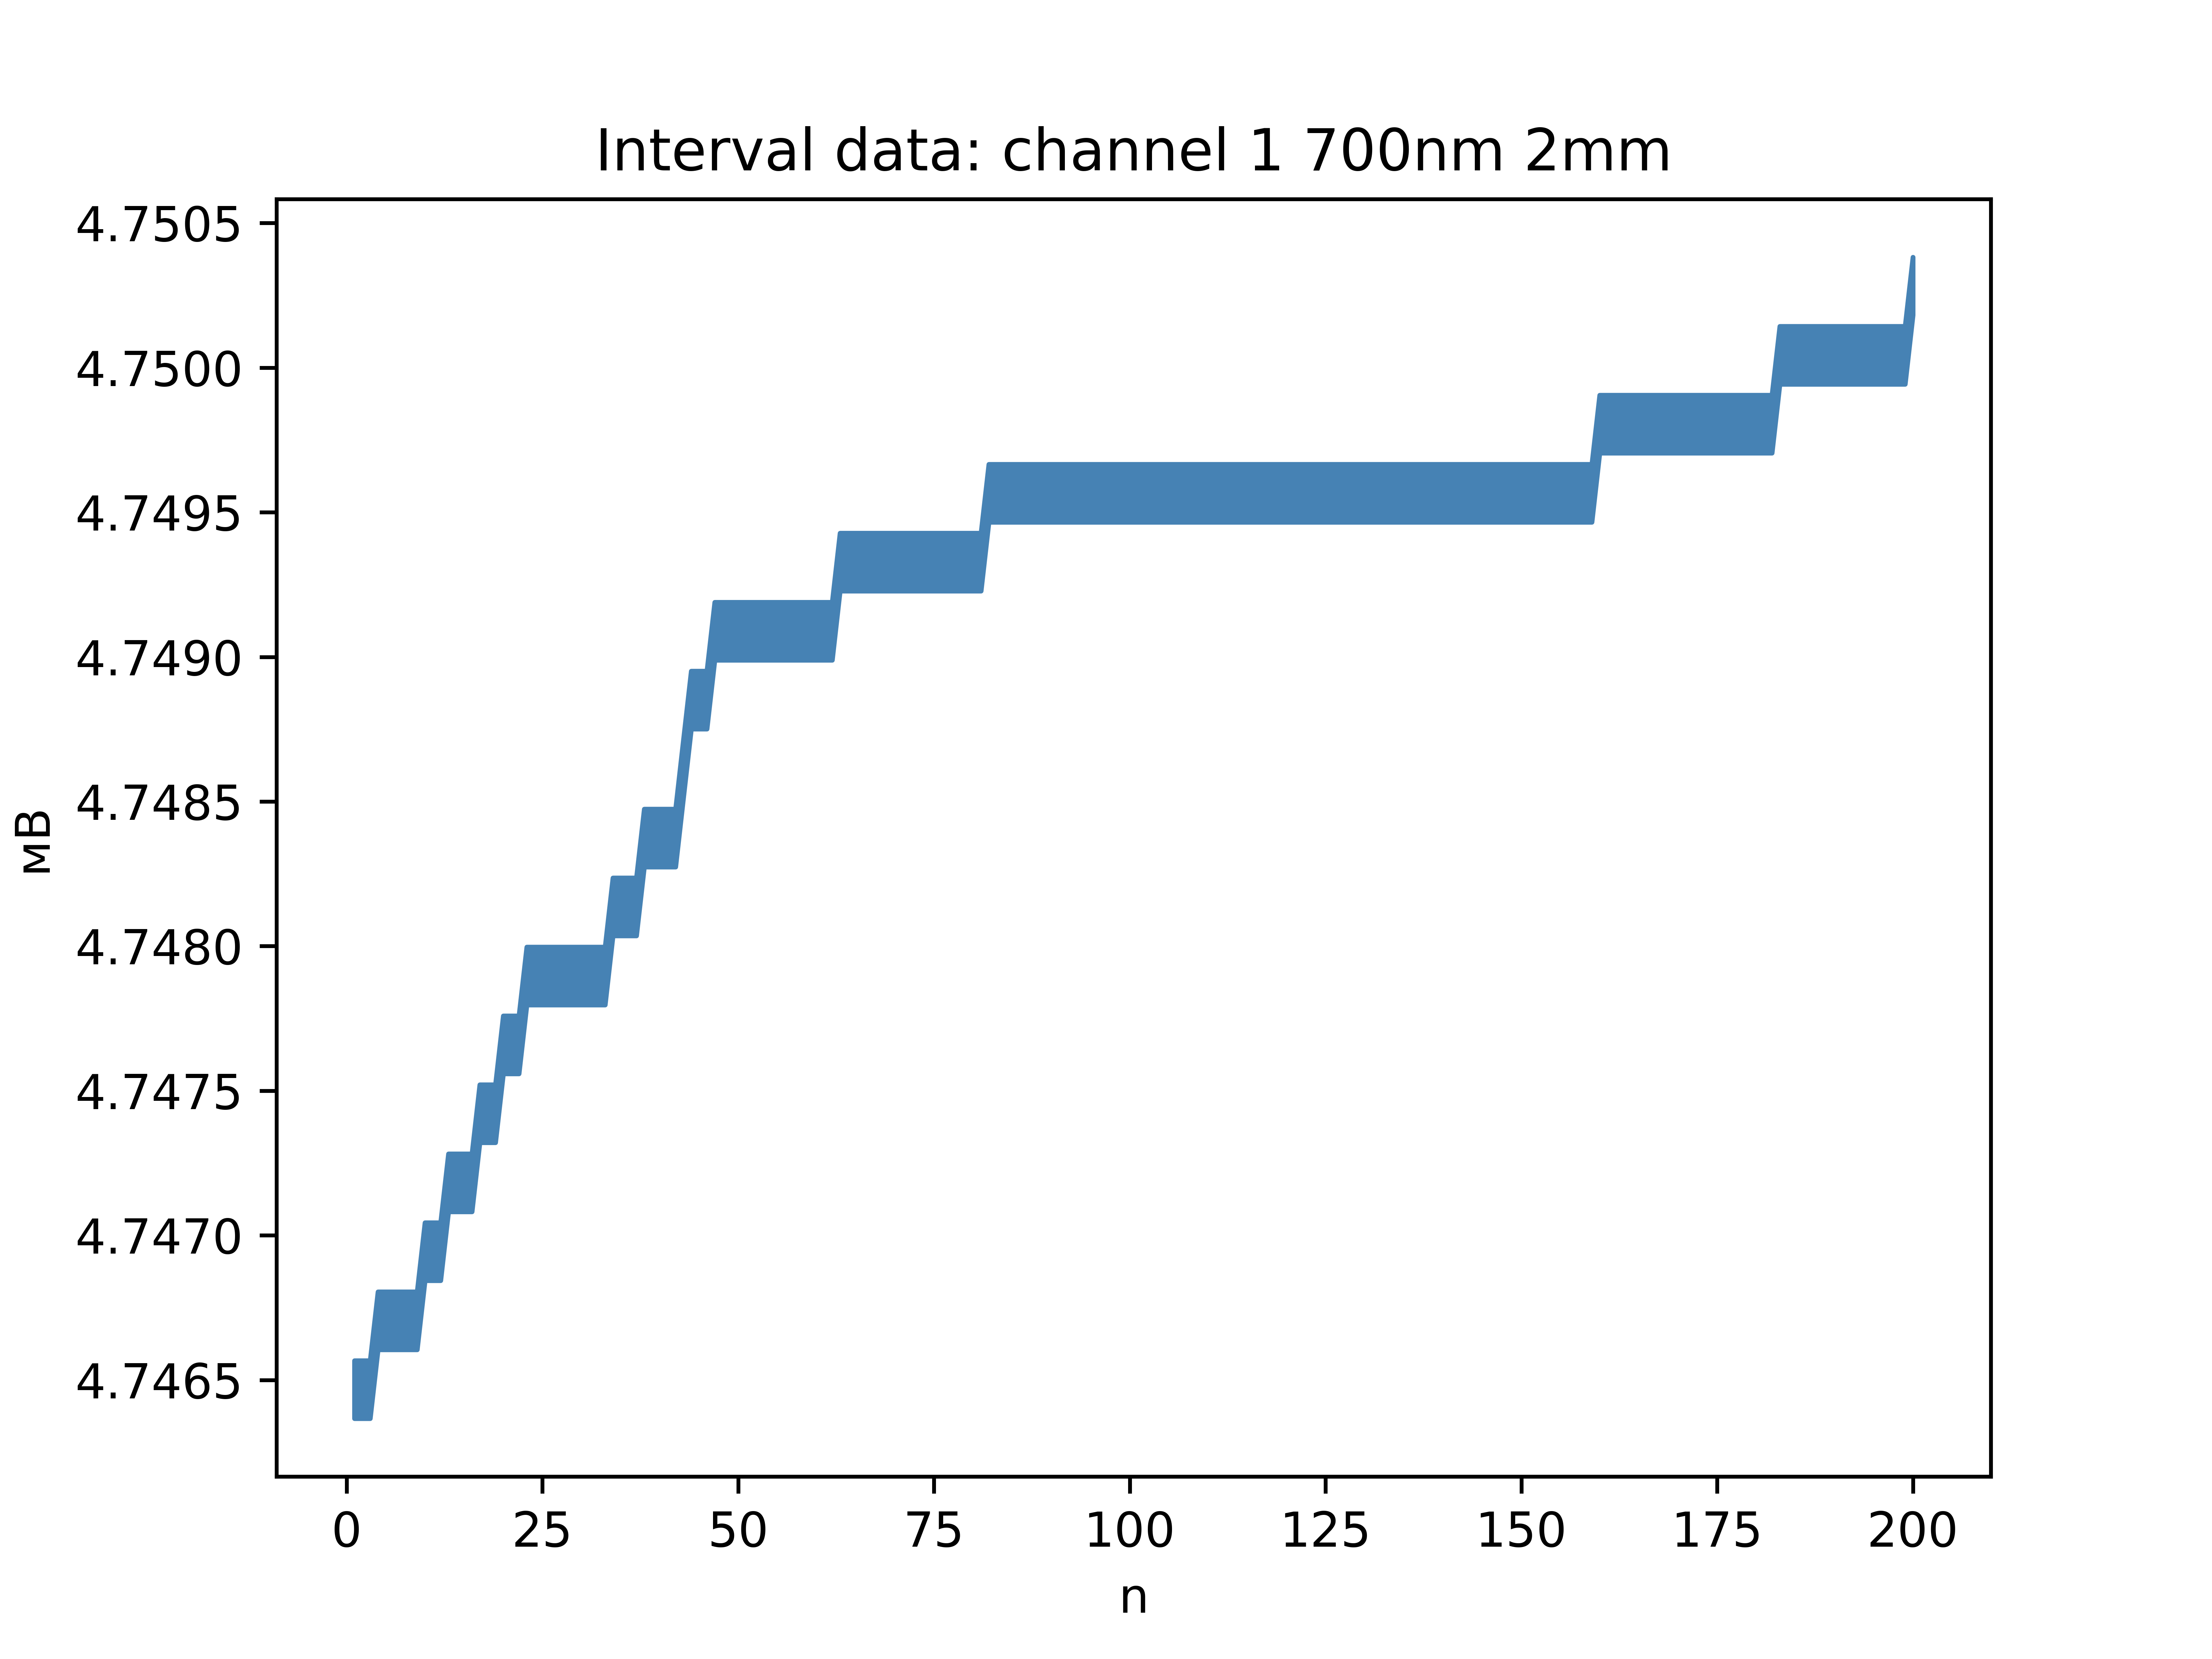
\includegraphics[scale=0.5]{resources/intervals_PR1.png}
		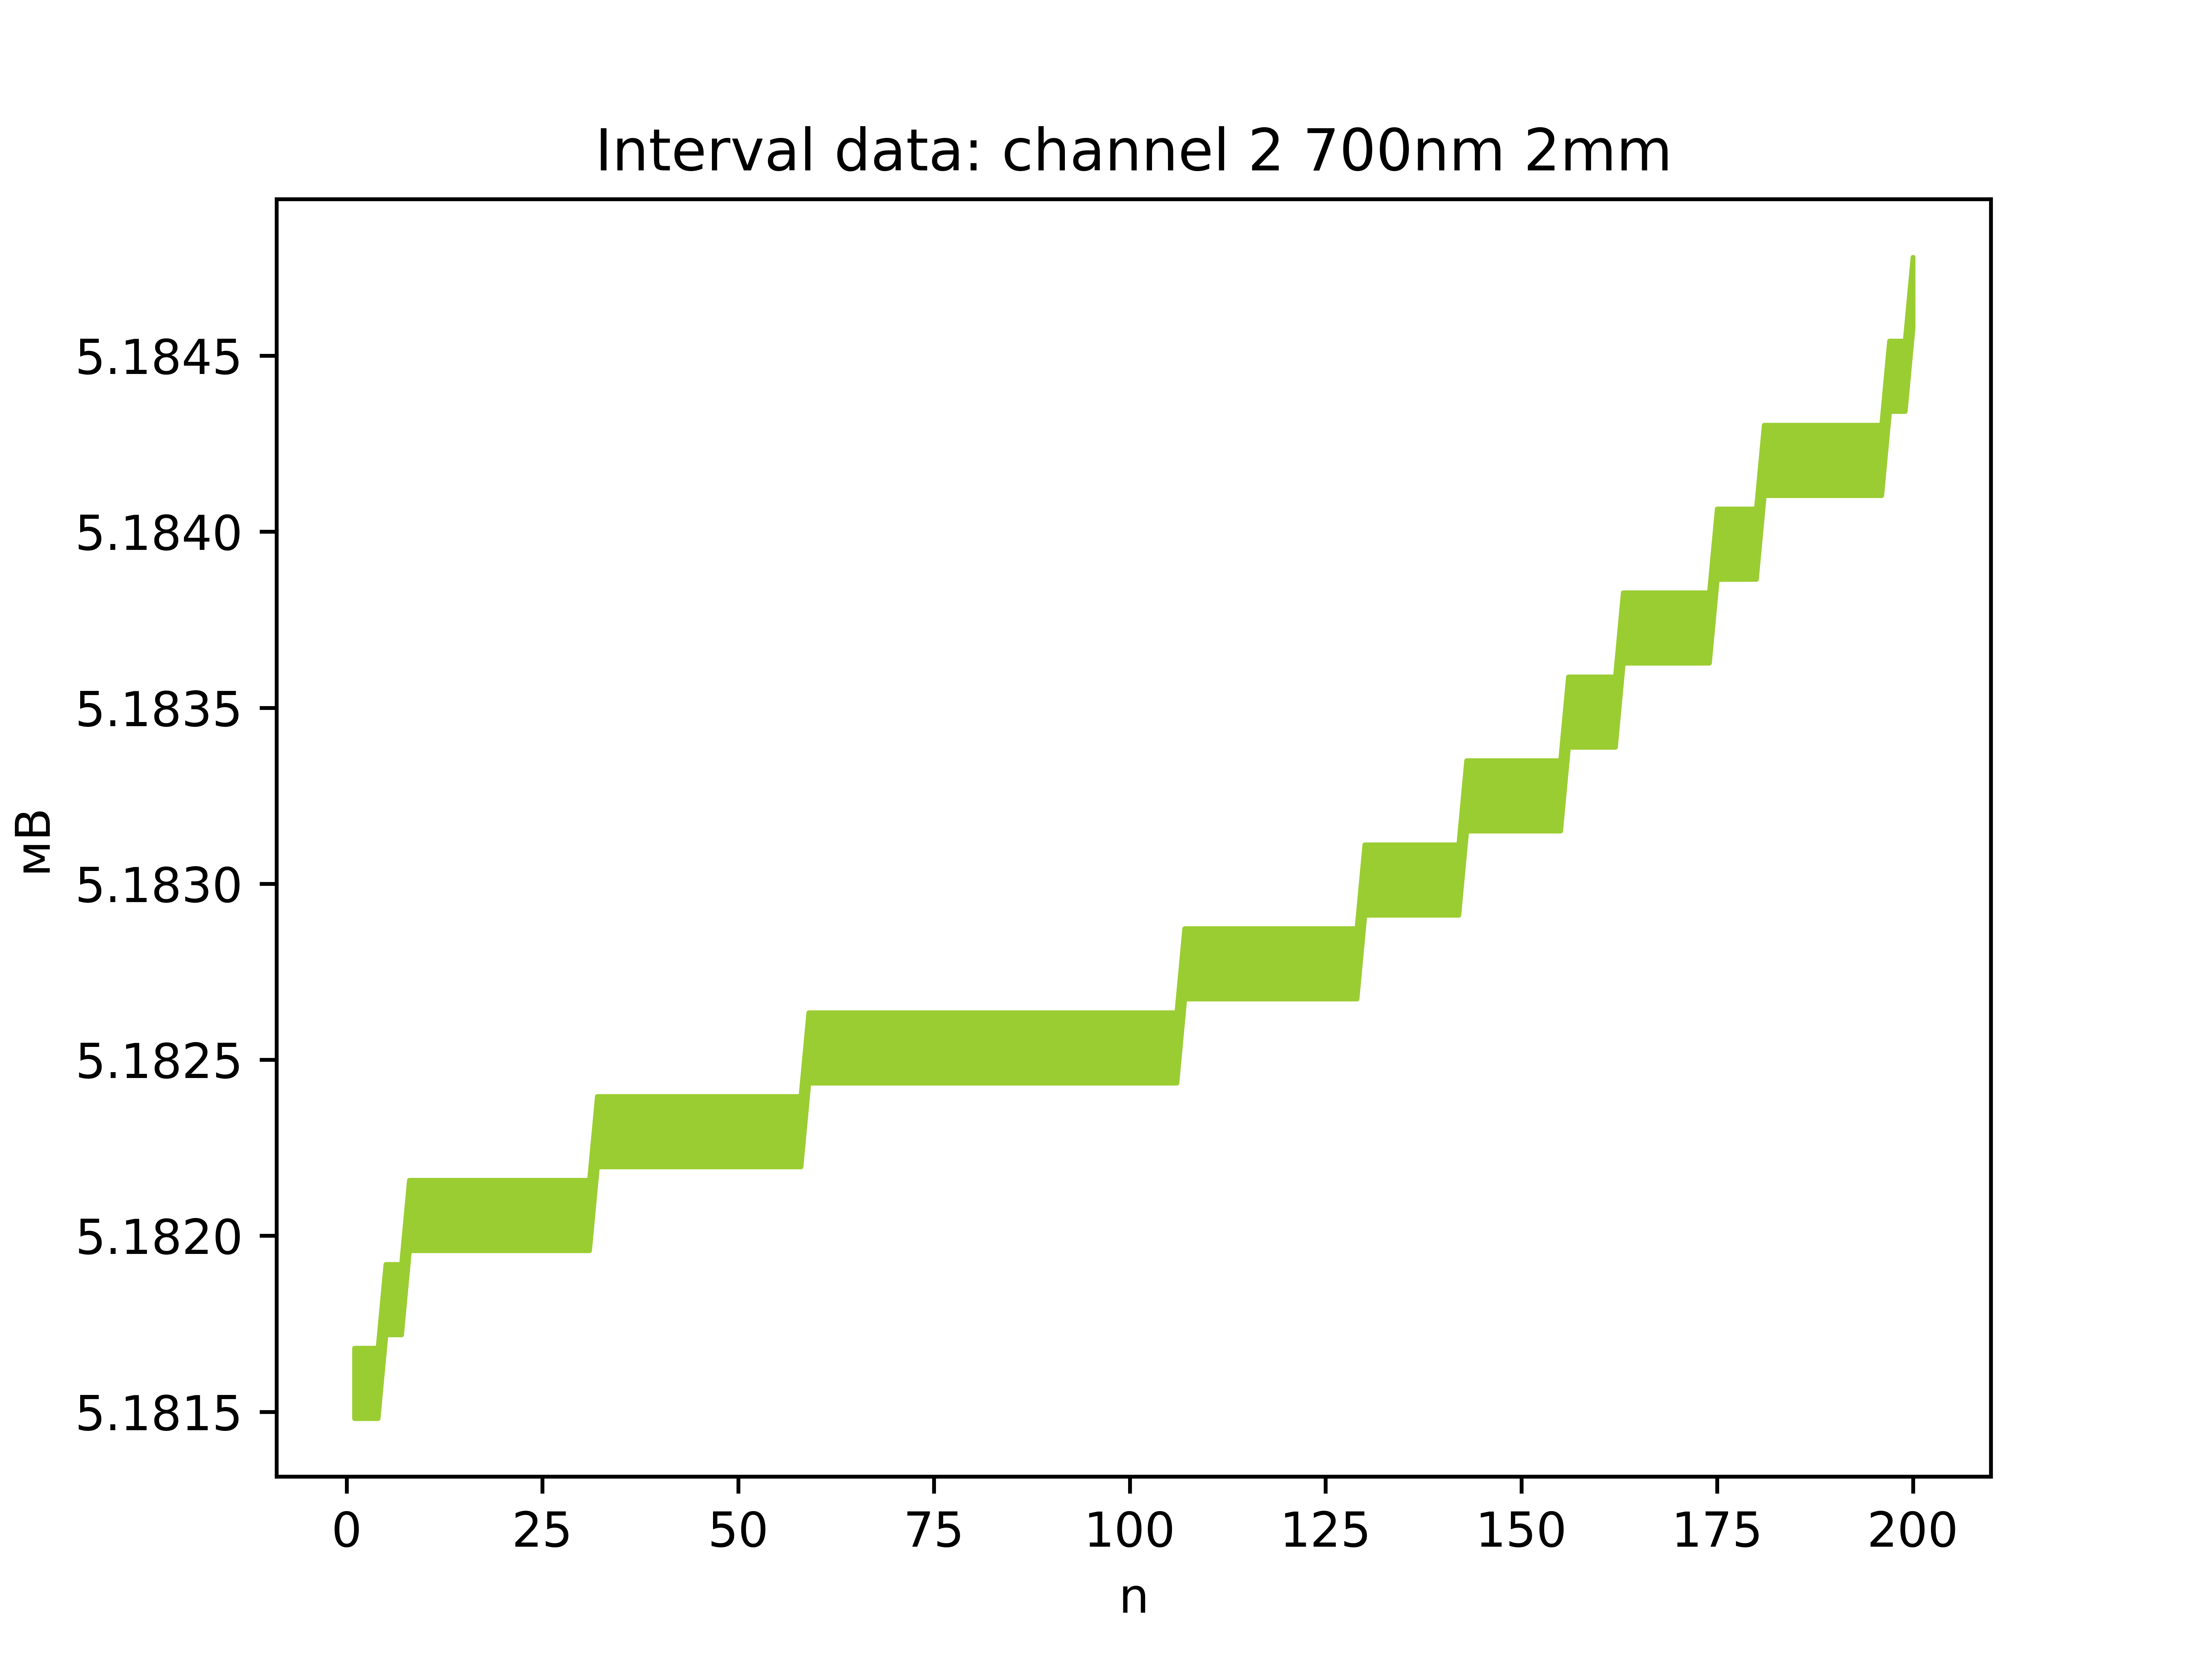
\includegraphics[scale=0.5]{resources/intervals_PR2.png}
	\end{tabular} \label{pic:intervals}
	\caption{Интервальное представление исходных данных} 
\end{figure}

\begin{figure}[H]
	\begin{tabular}{ccc}
		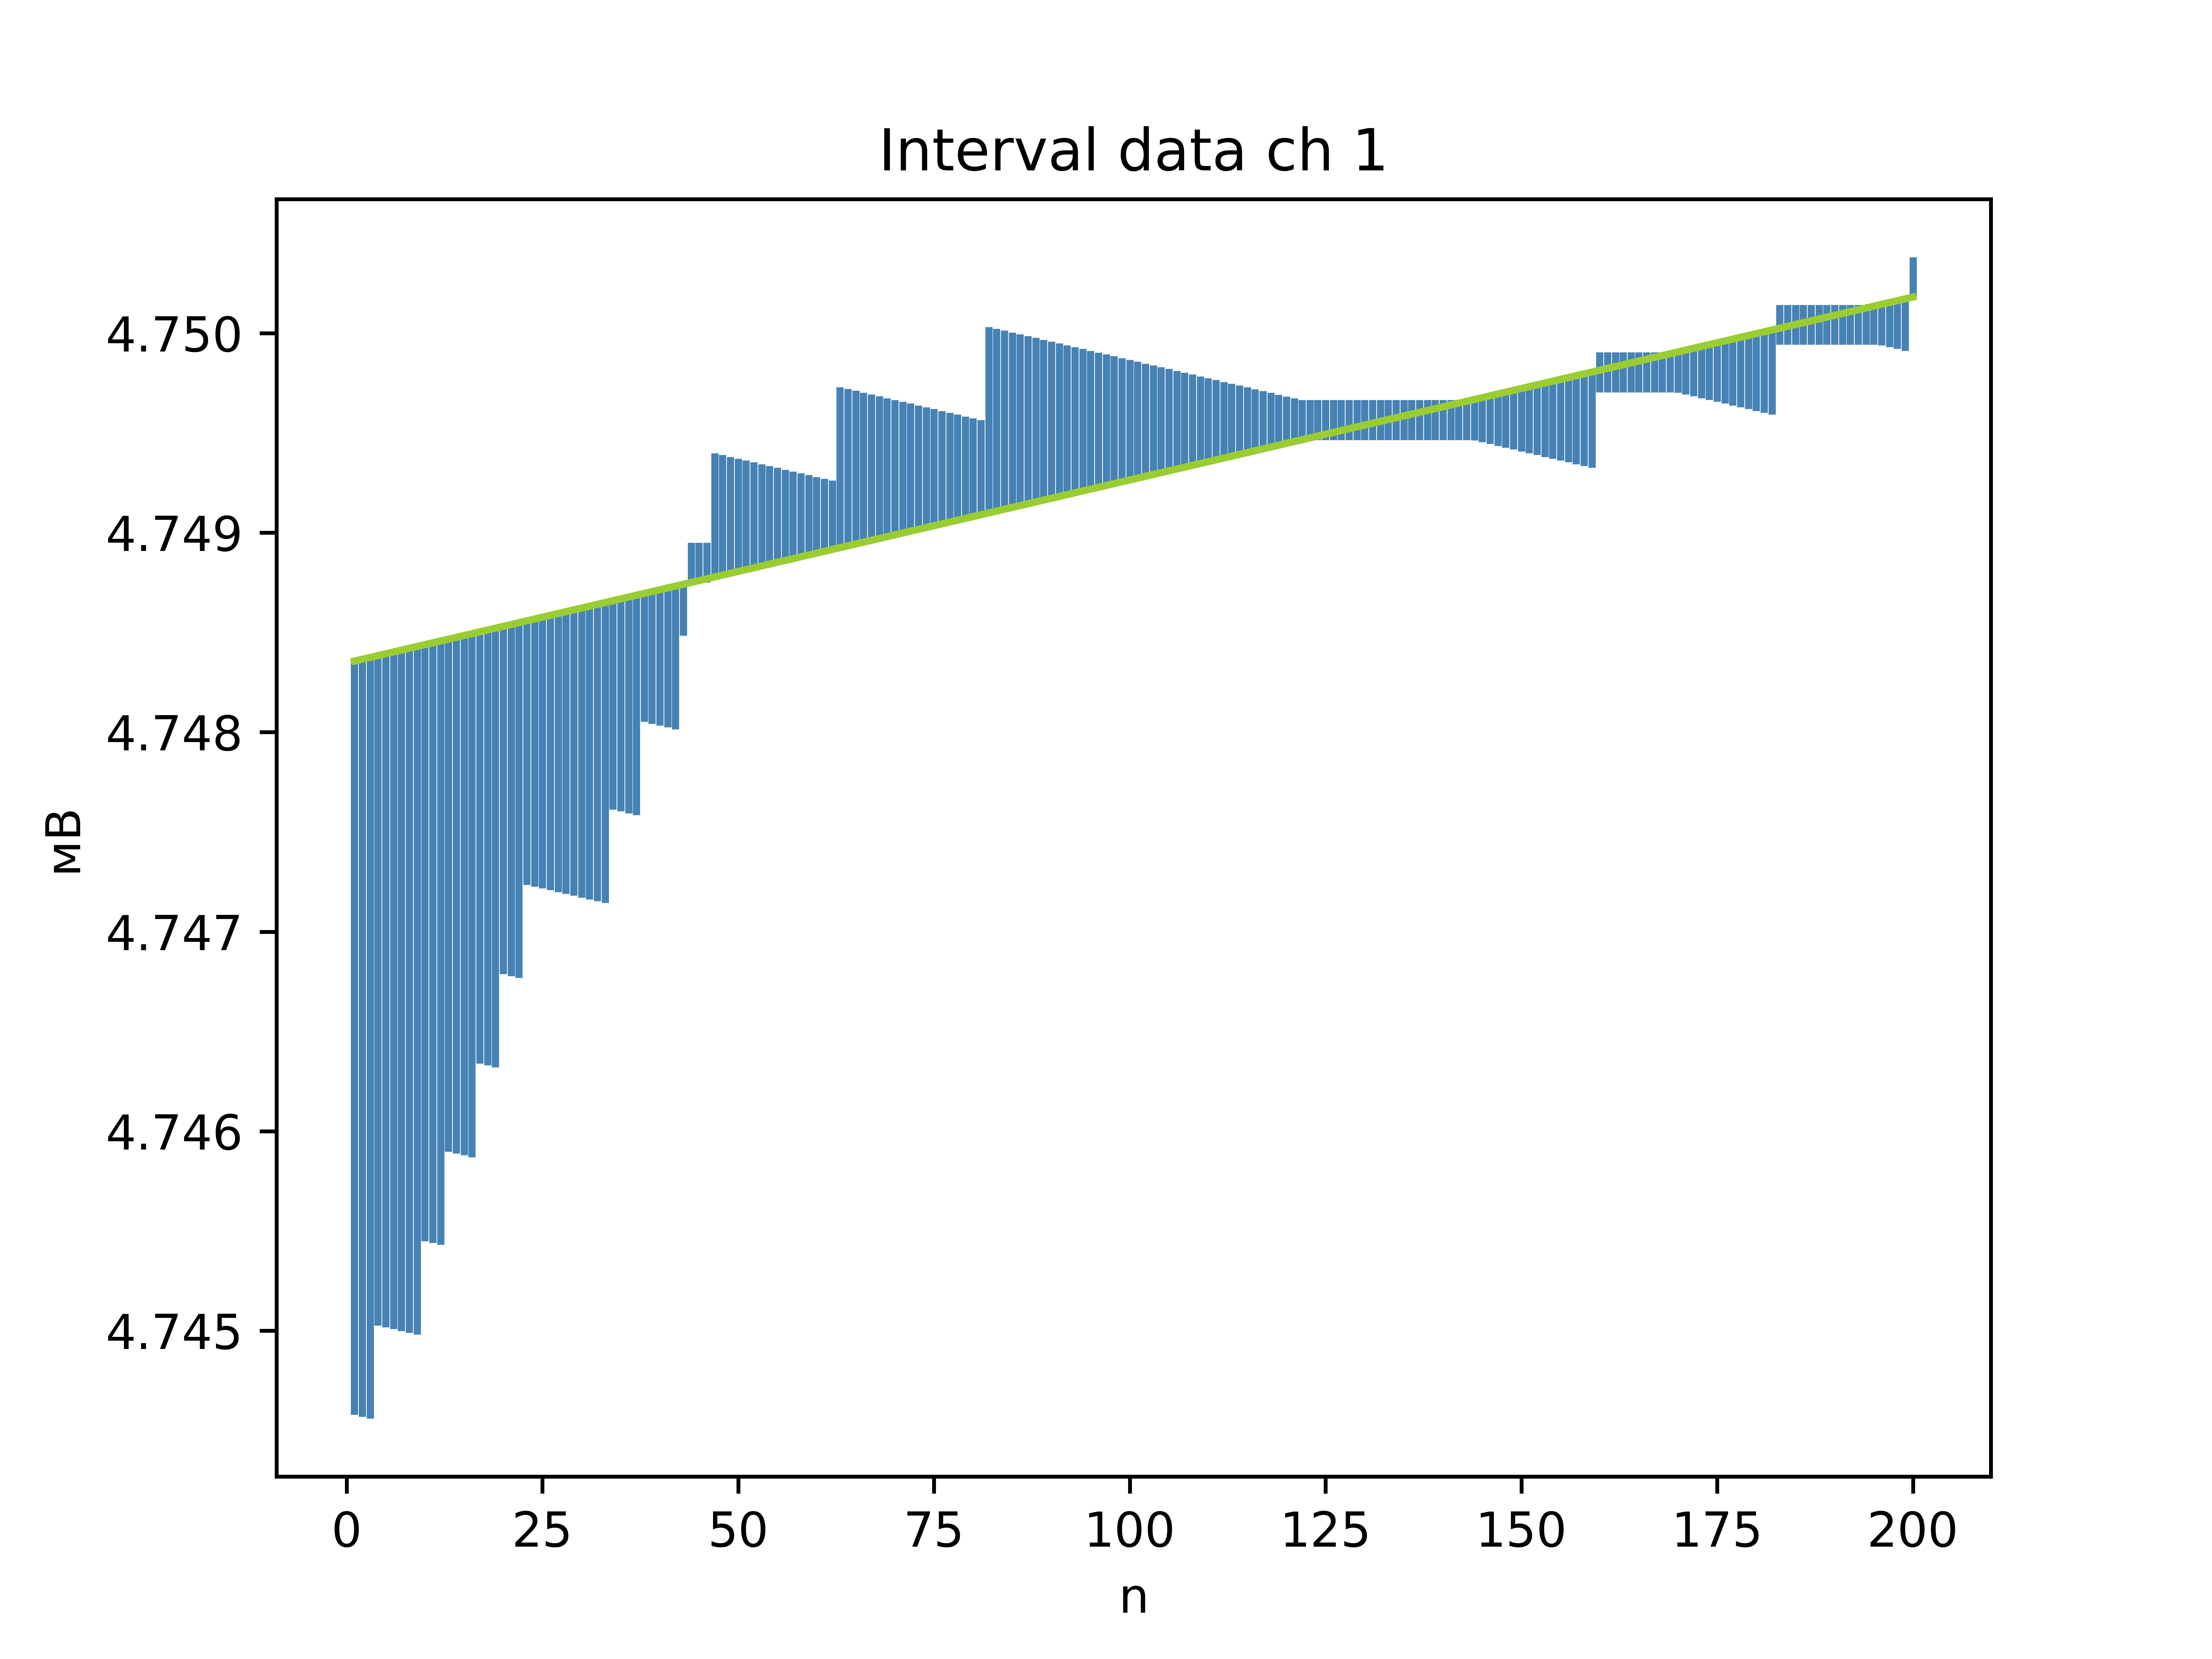
\includegraphics[scale=0.5]{resources/lr_PR1.png}
		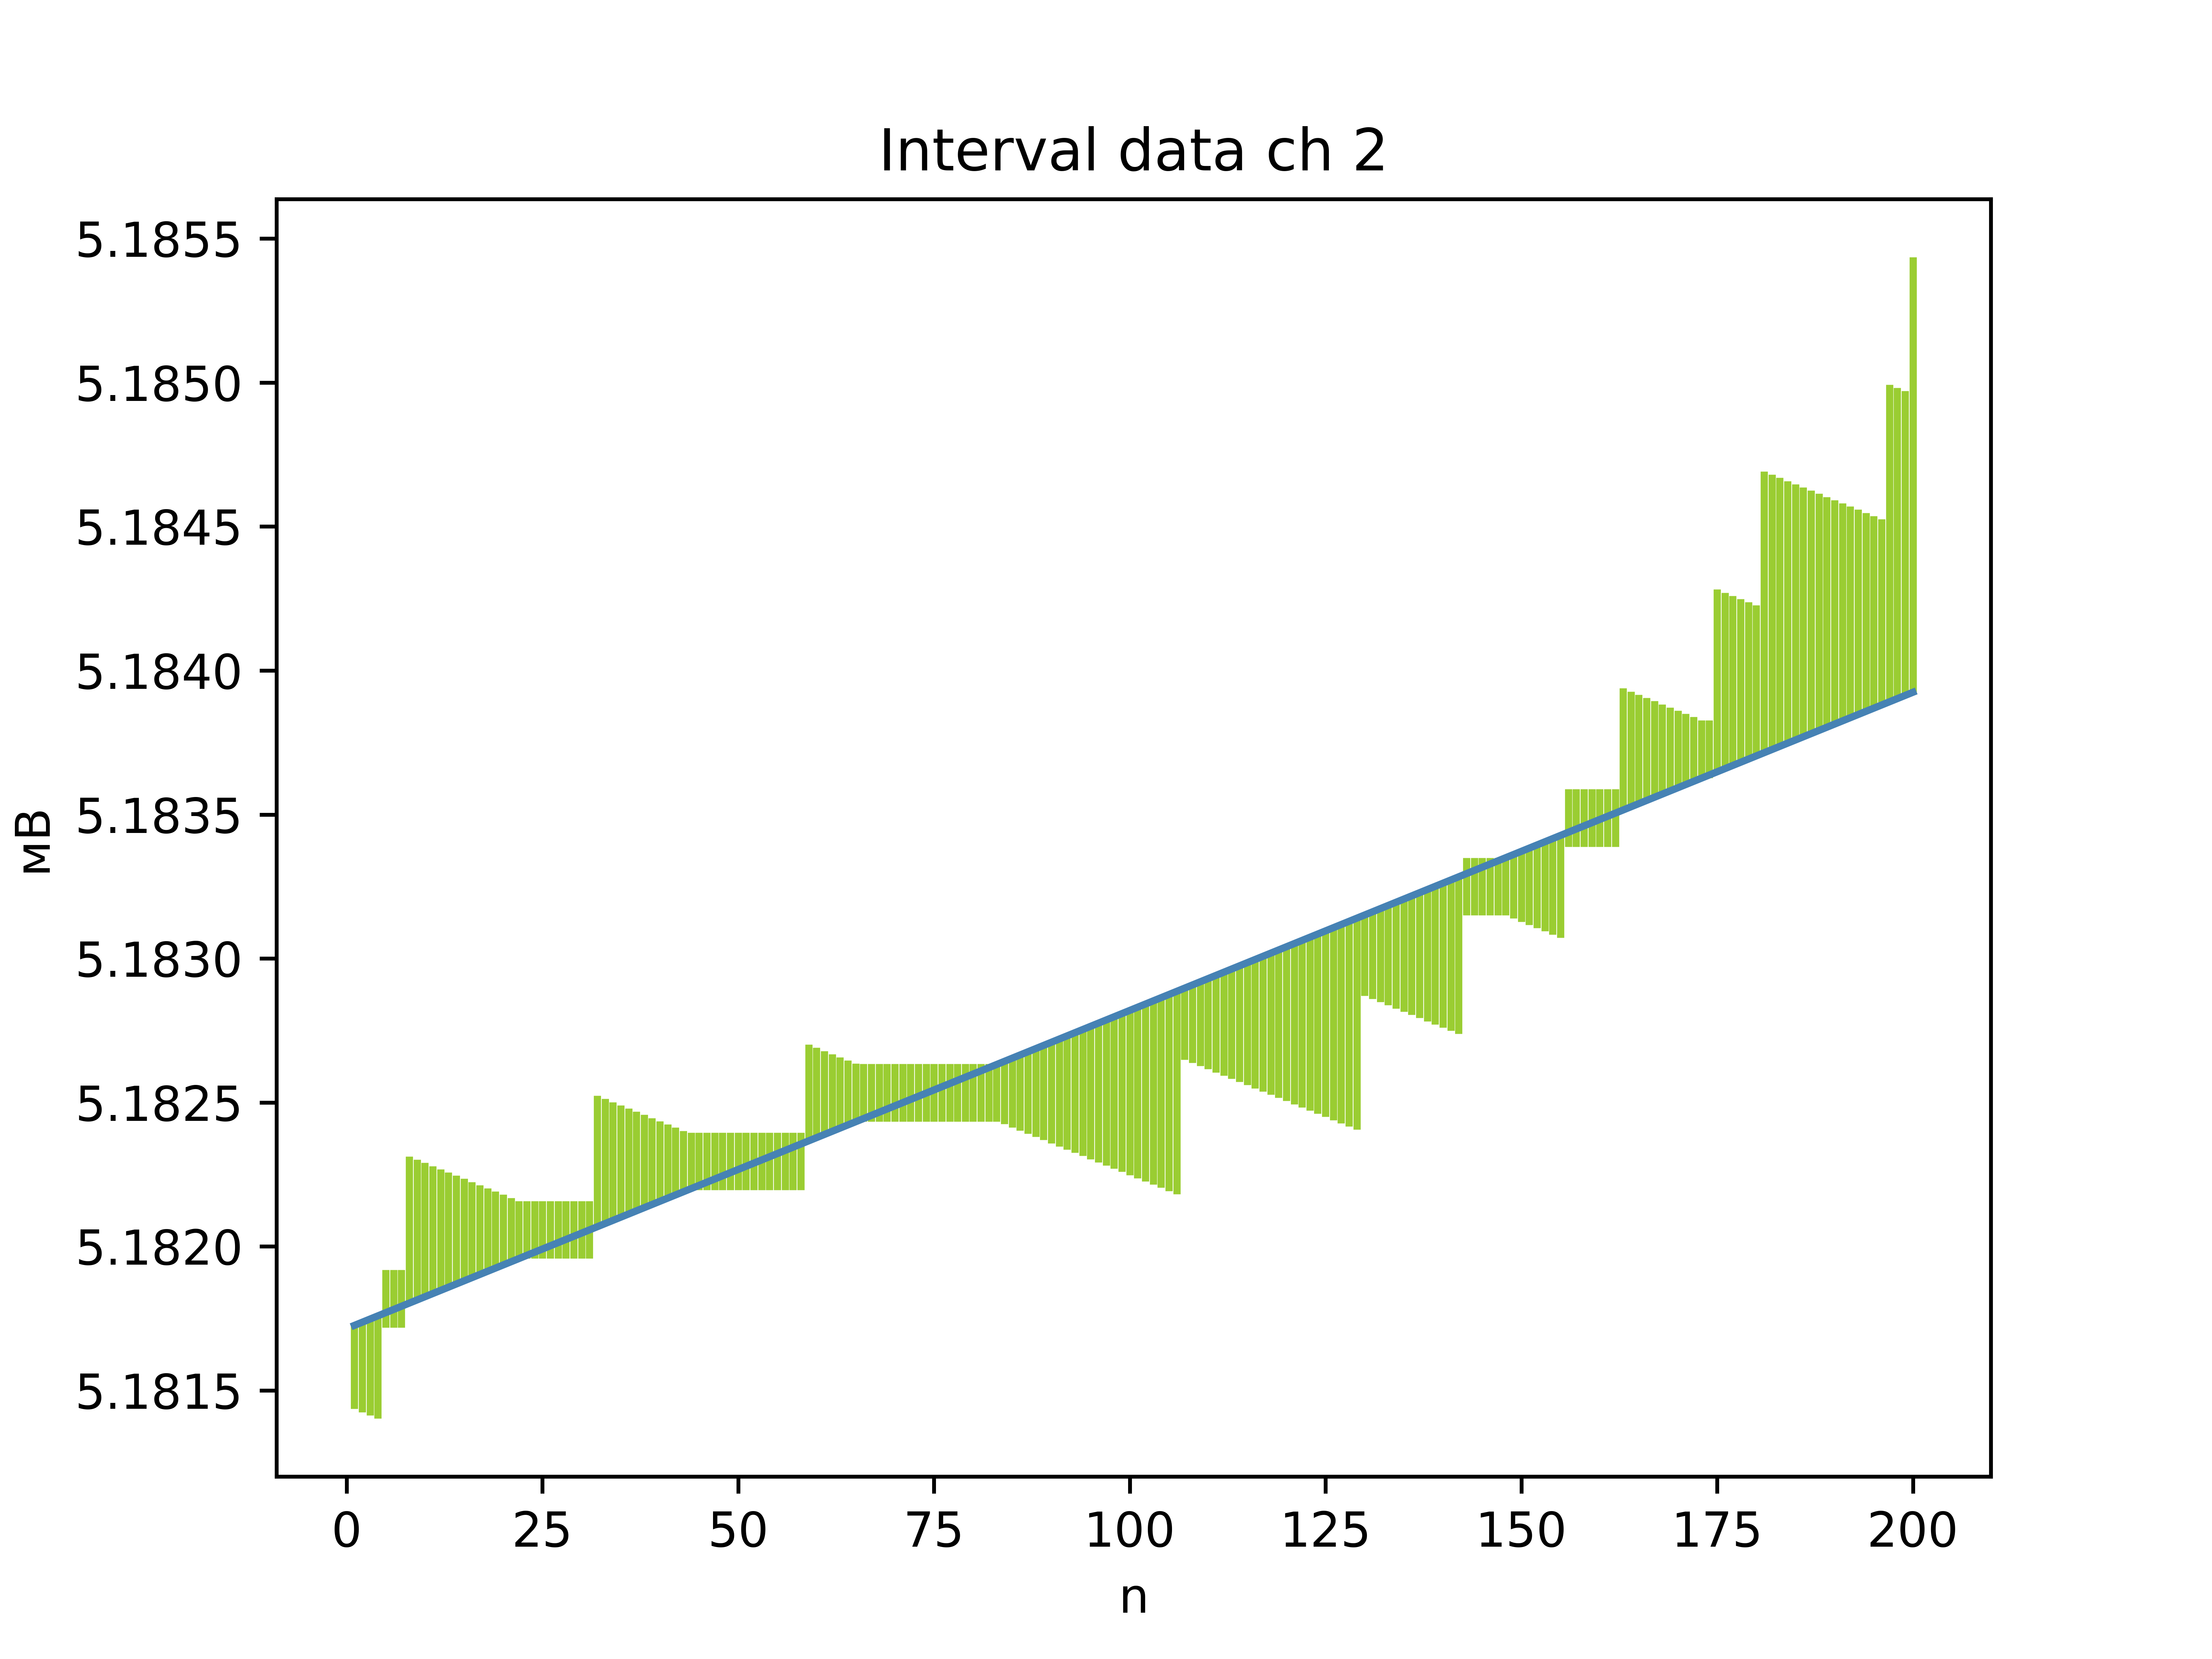
\includegraphics[scale=0.5]{resources/lr_PR2.png}
	\end{tabular}
	\caption{Линейная модель дрейфа данных} 
\end{figure}

\begin{figure}[H]
	\begin{tabular}{ccc}
		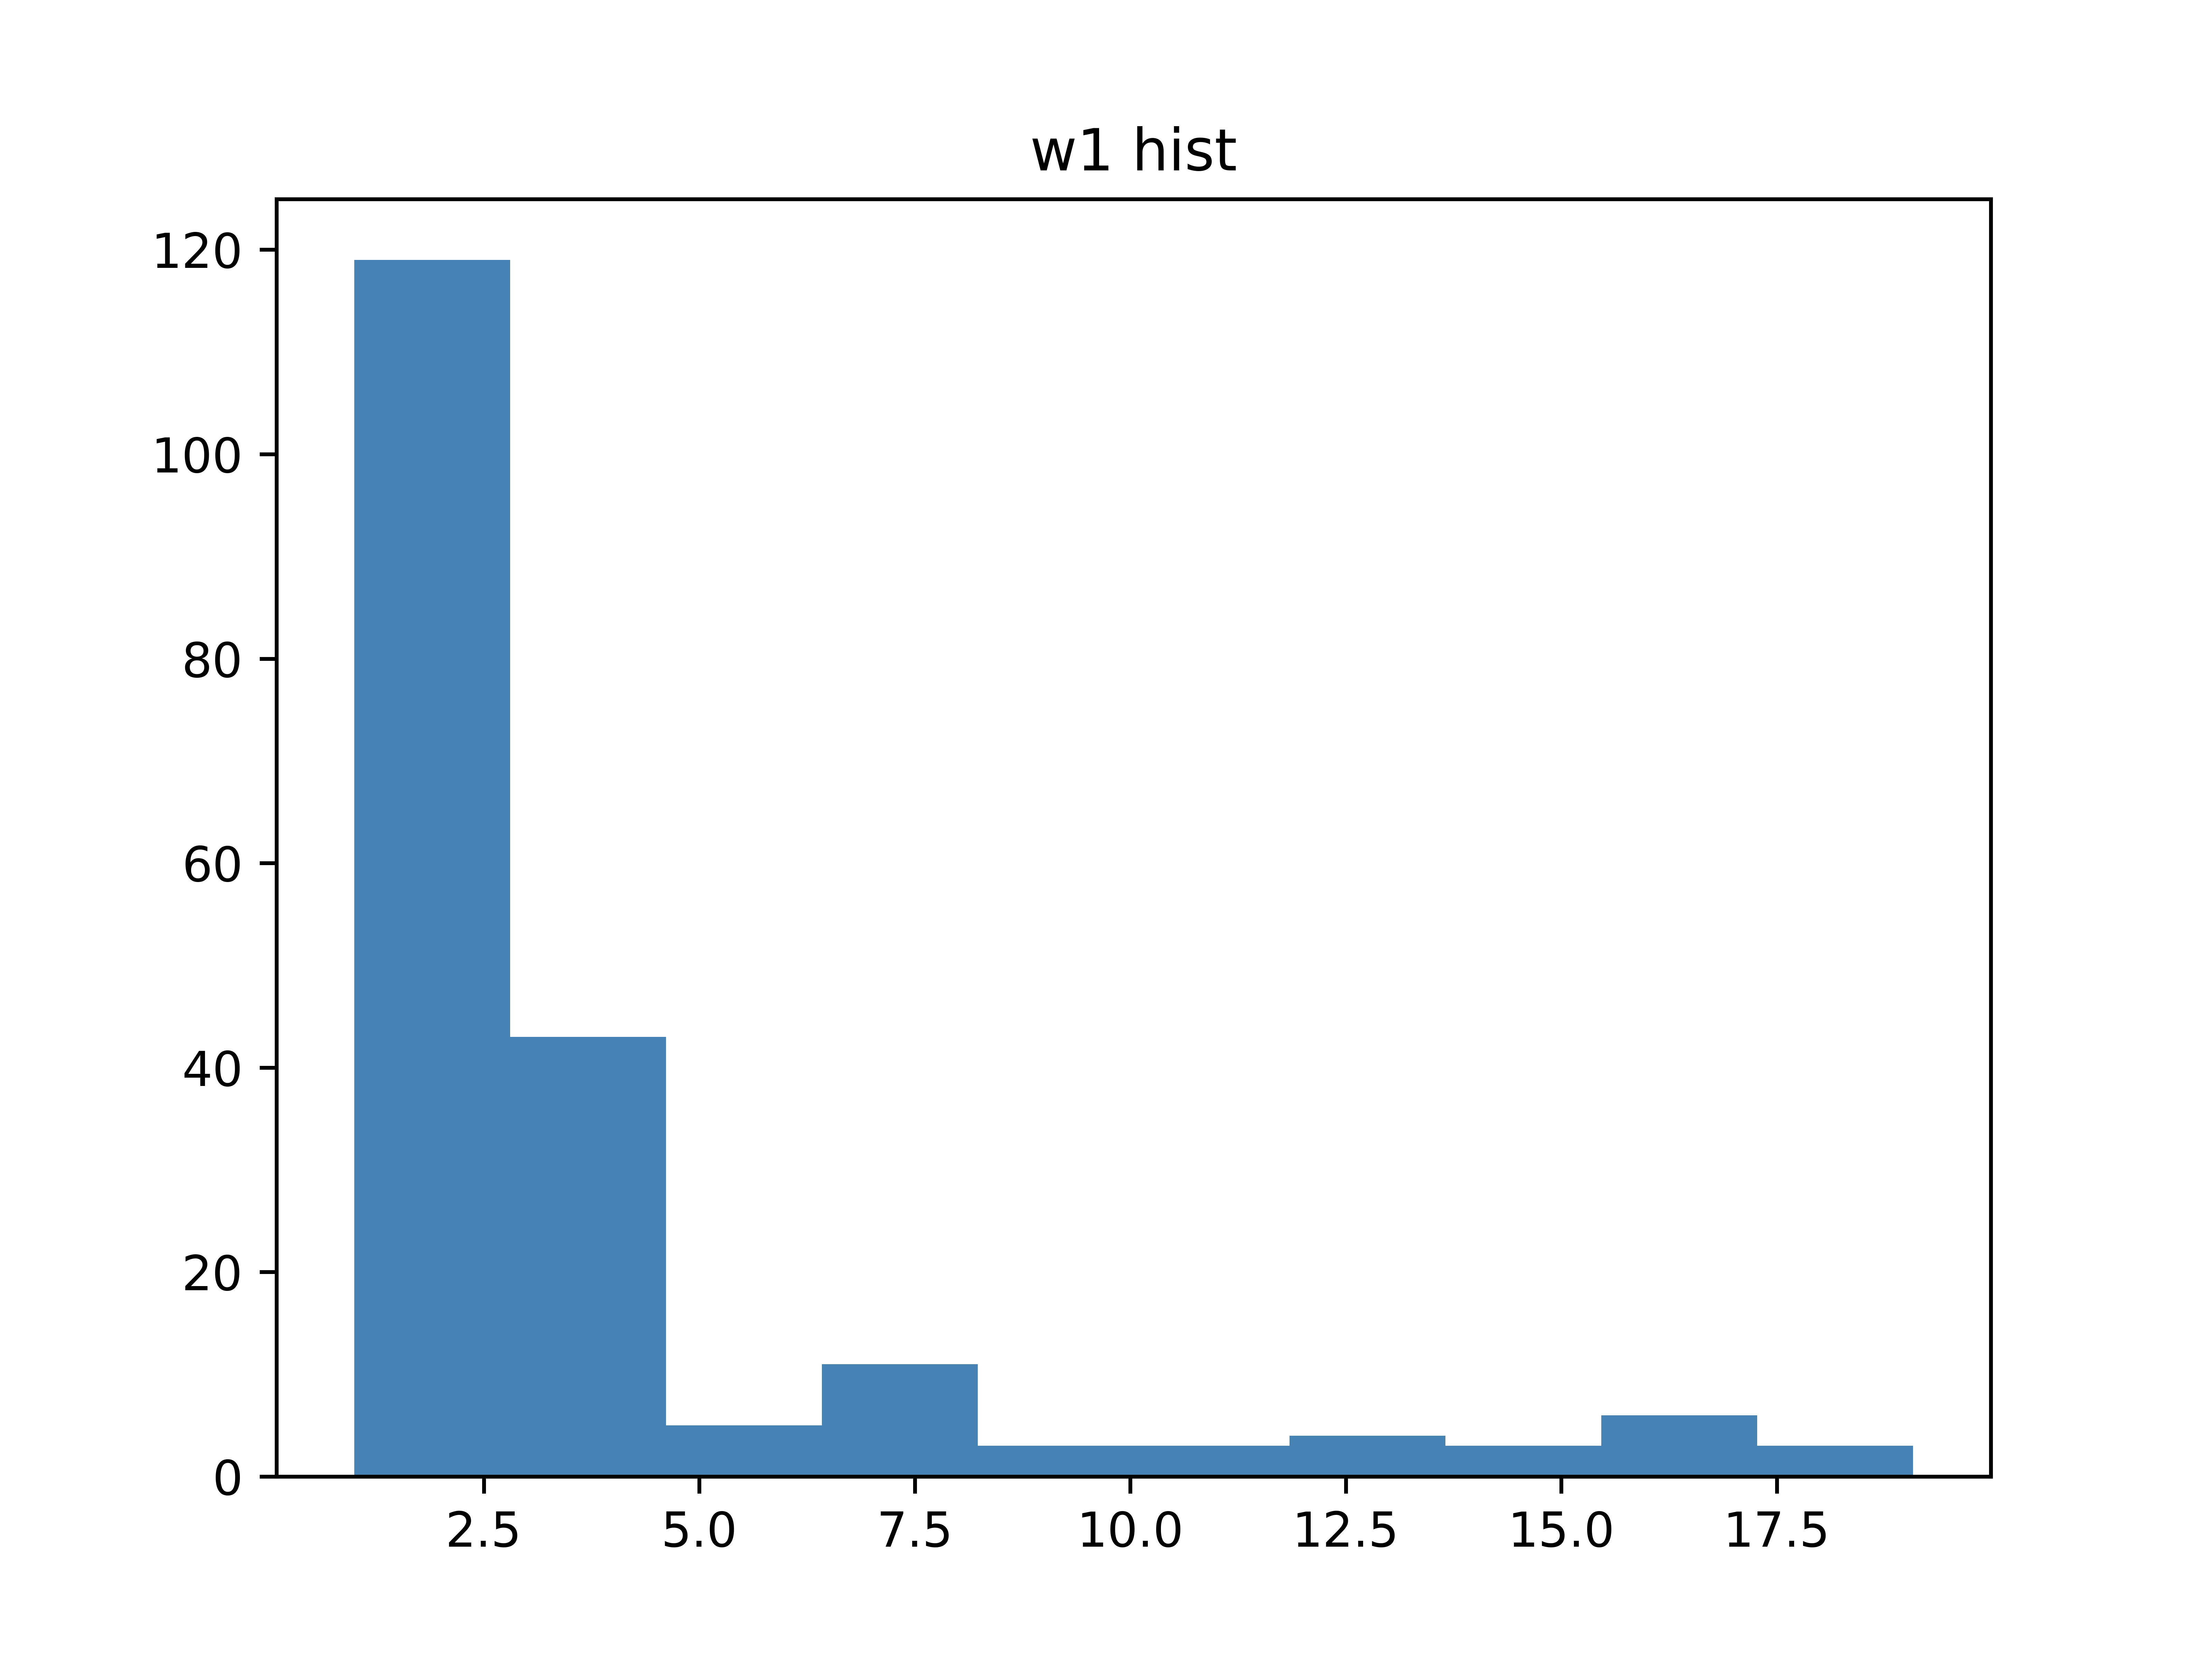
\includegraphics[scale=0.5]{resources/whyst_PR1.png}
		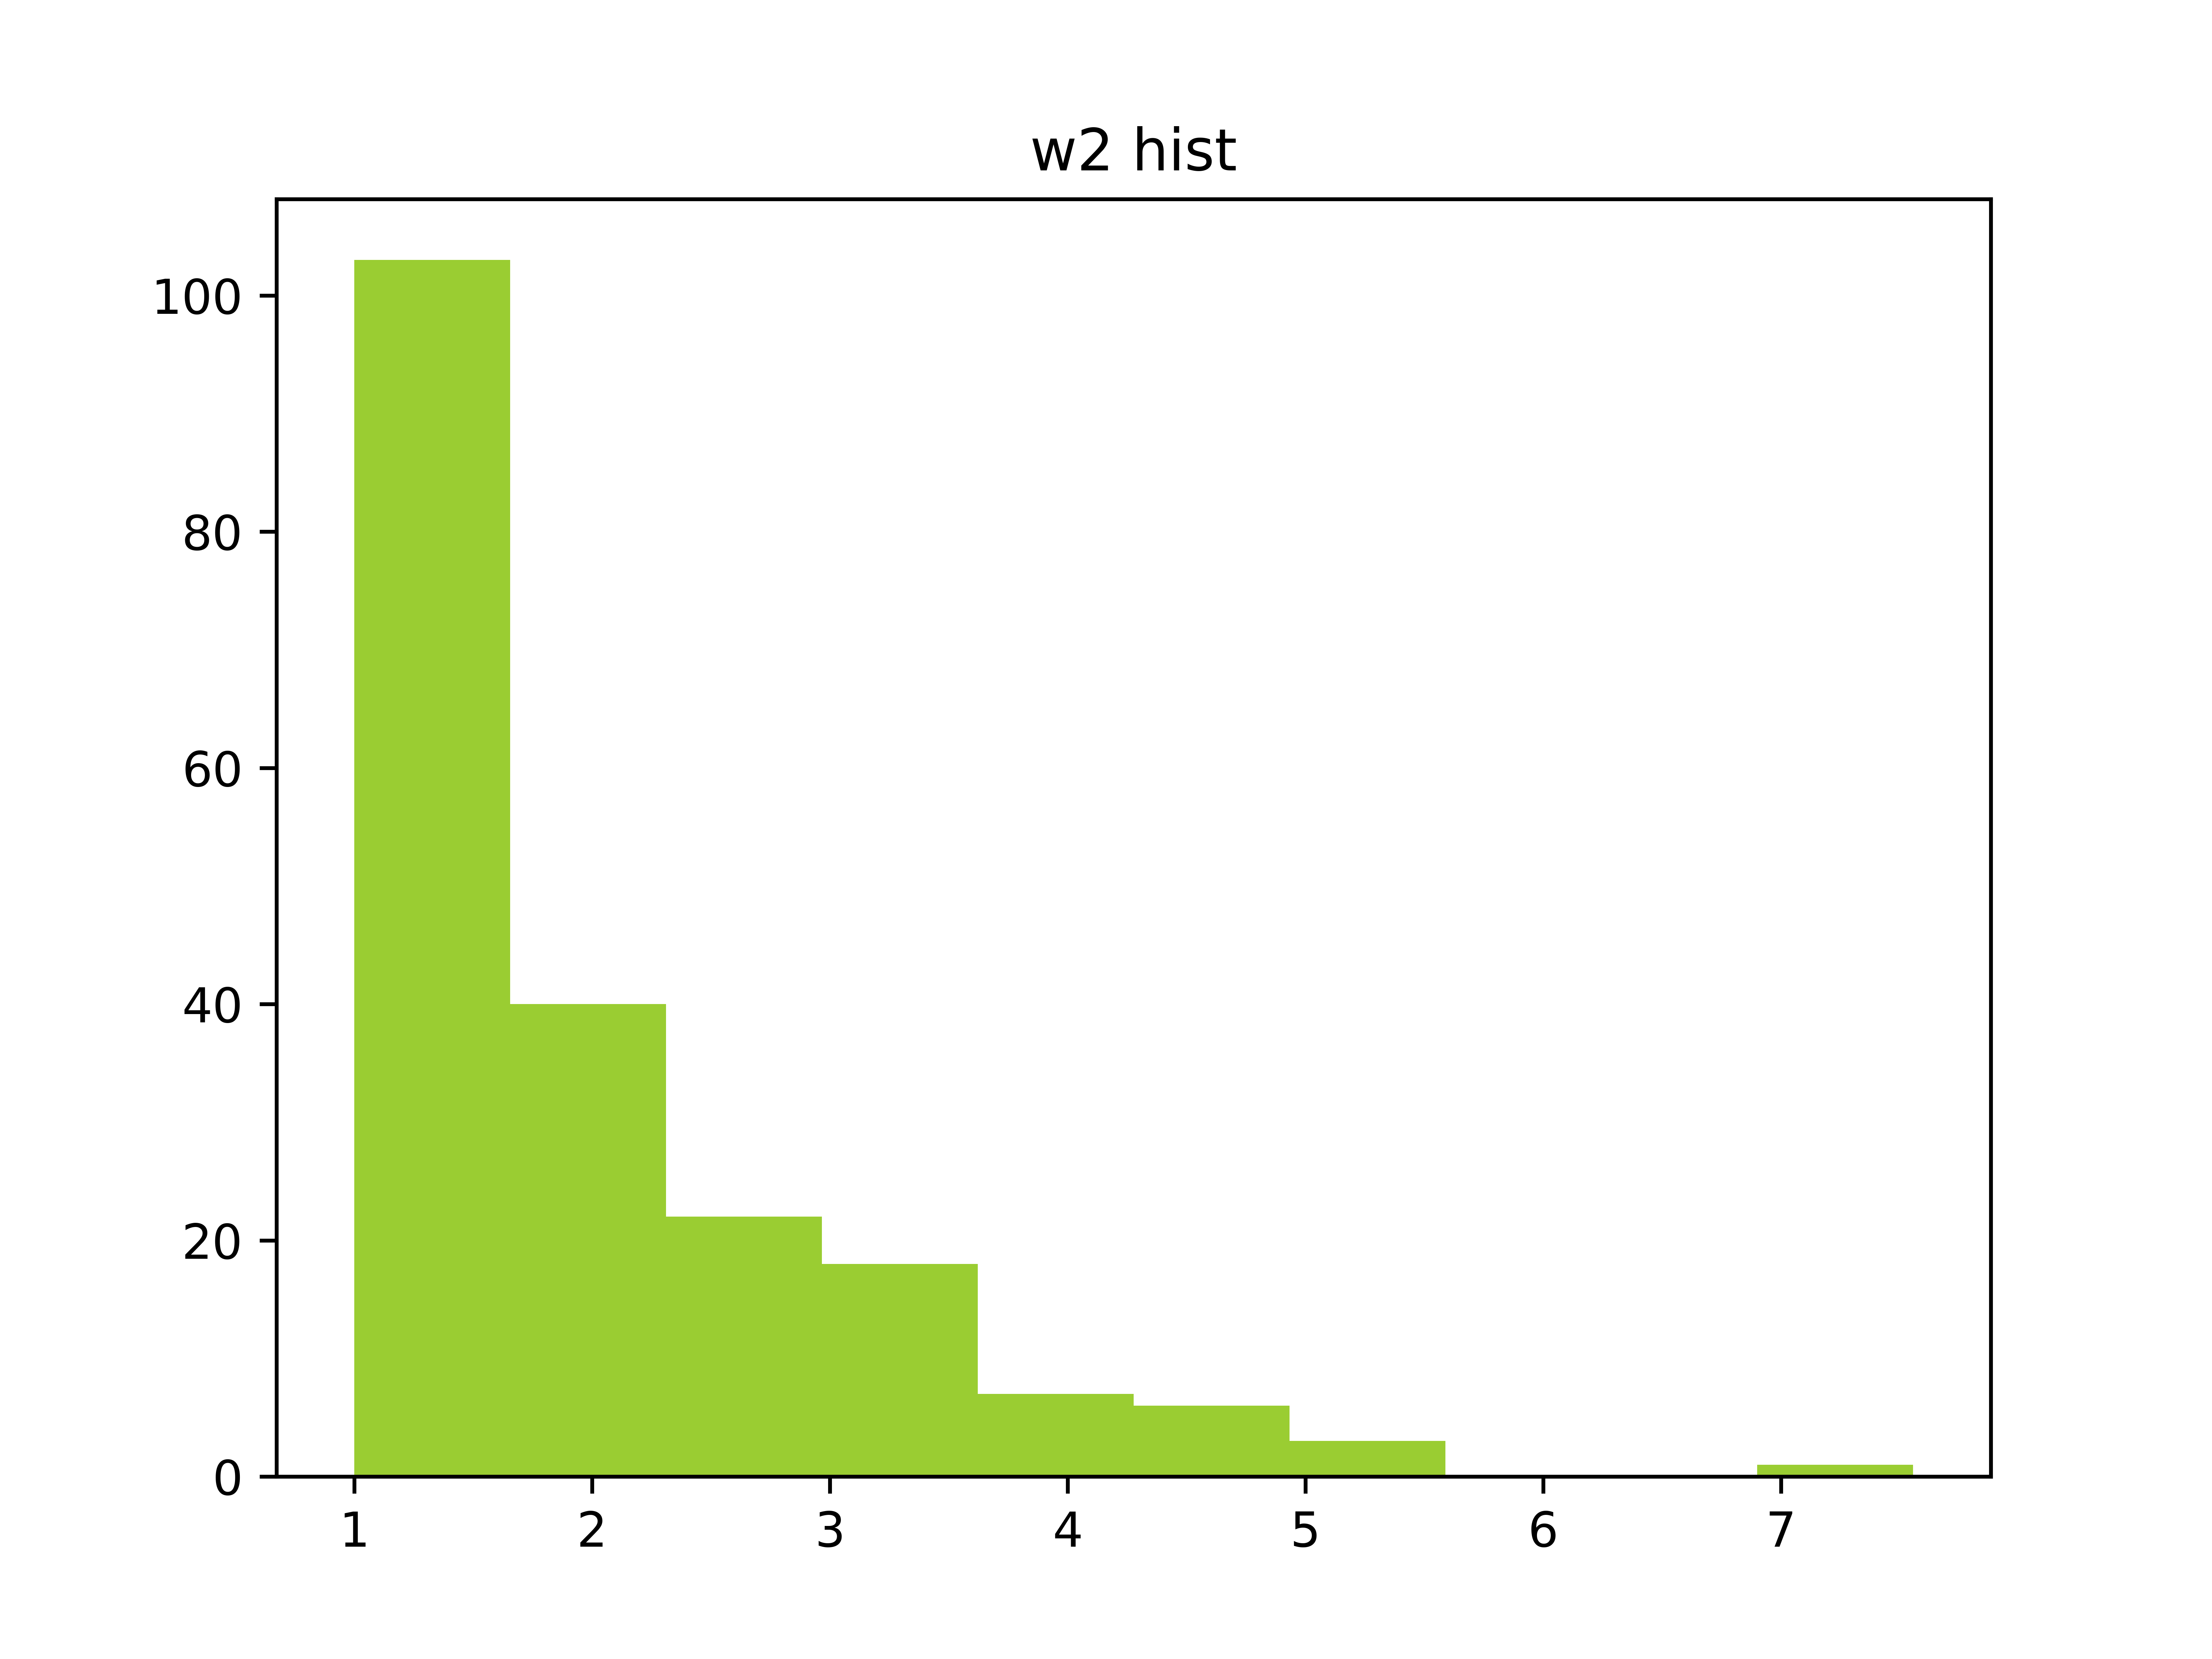
\includegraphics[scale=0.5]{resources/whyst_PR2.png}
	\end{tabular} \label{pic:whysts}
	\caption{Гистограммы значений множителей коррекции w} 
\end{figure}

\begin{figure}[H]
	\begin{tabular}{ccc}
		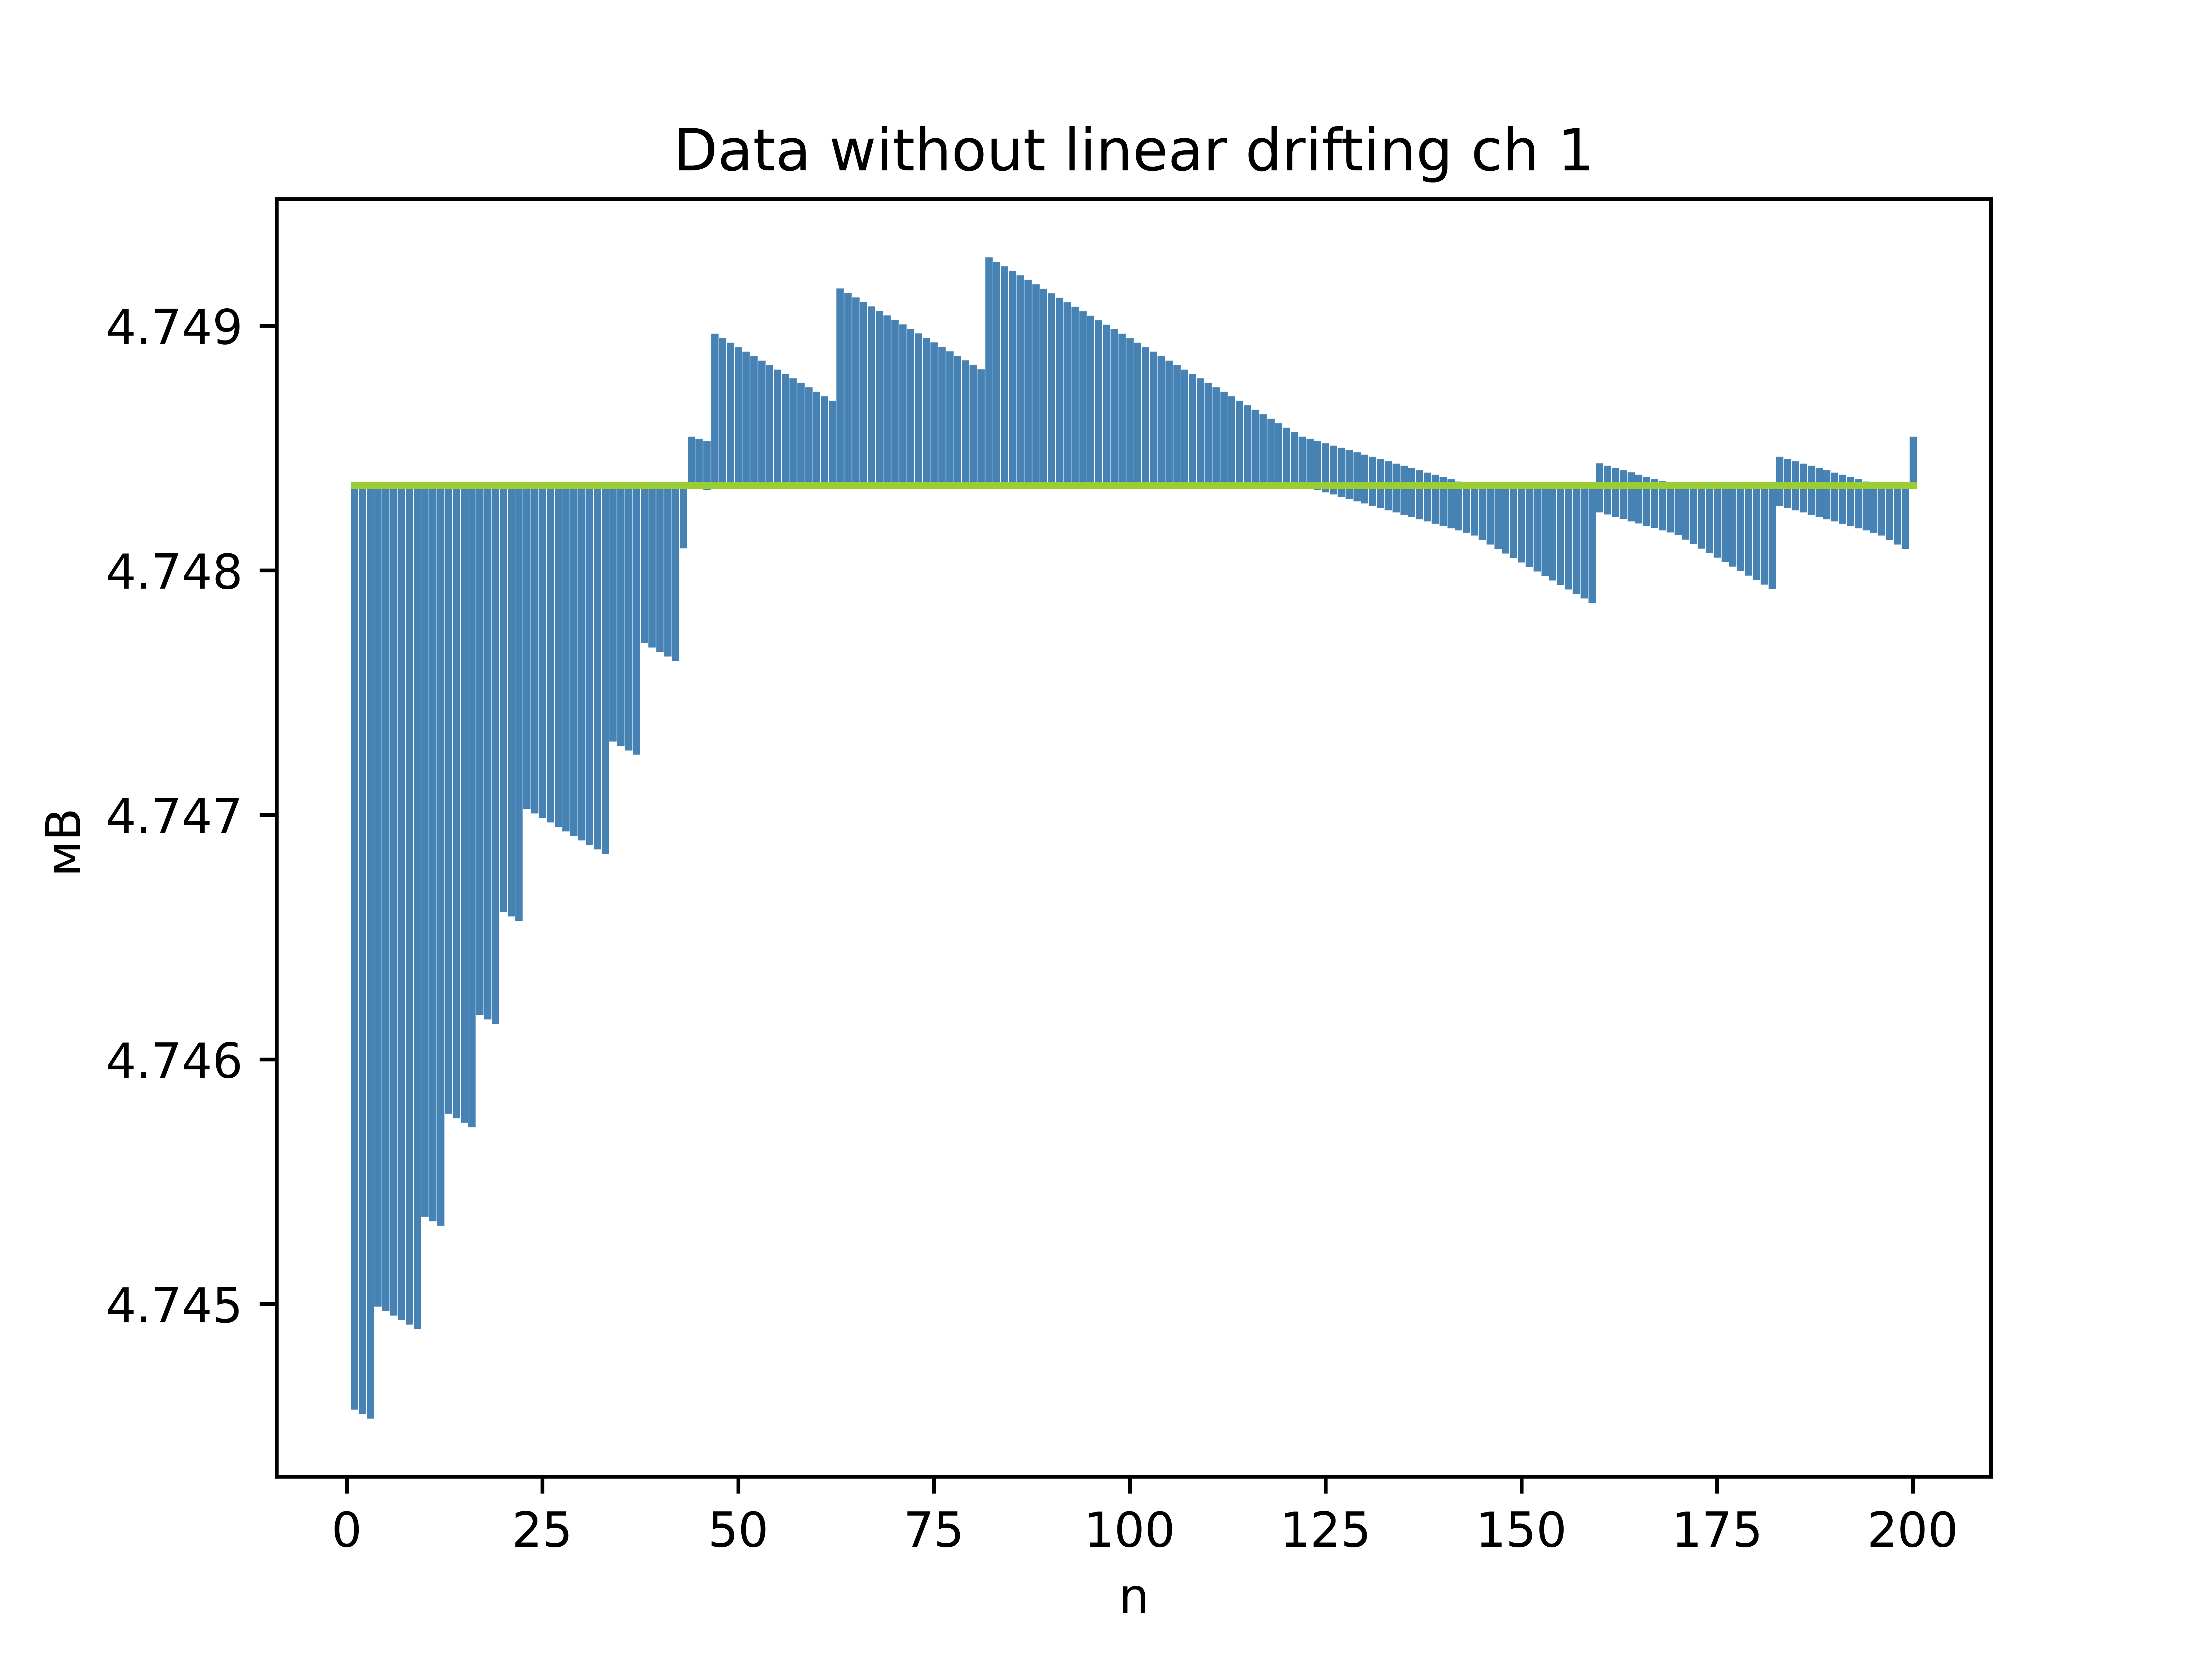
\includegraphics[scale=0.5]{resources/fixed_PR1.png}
		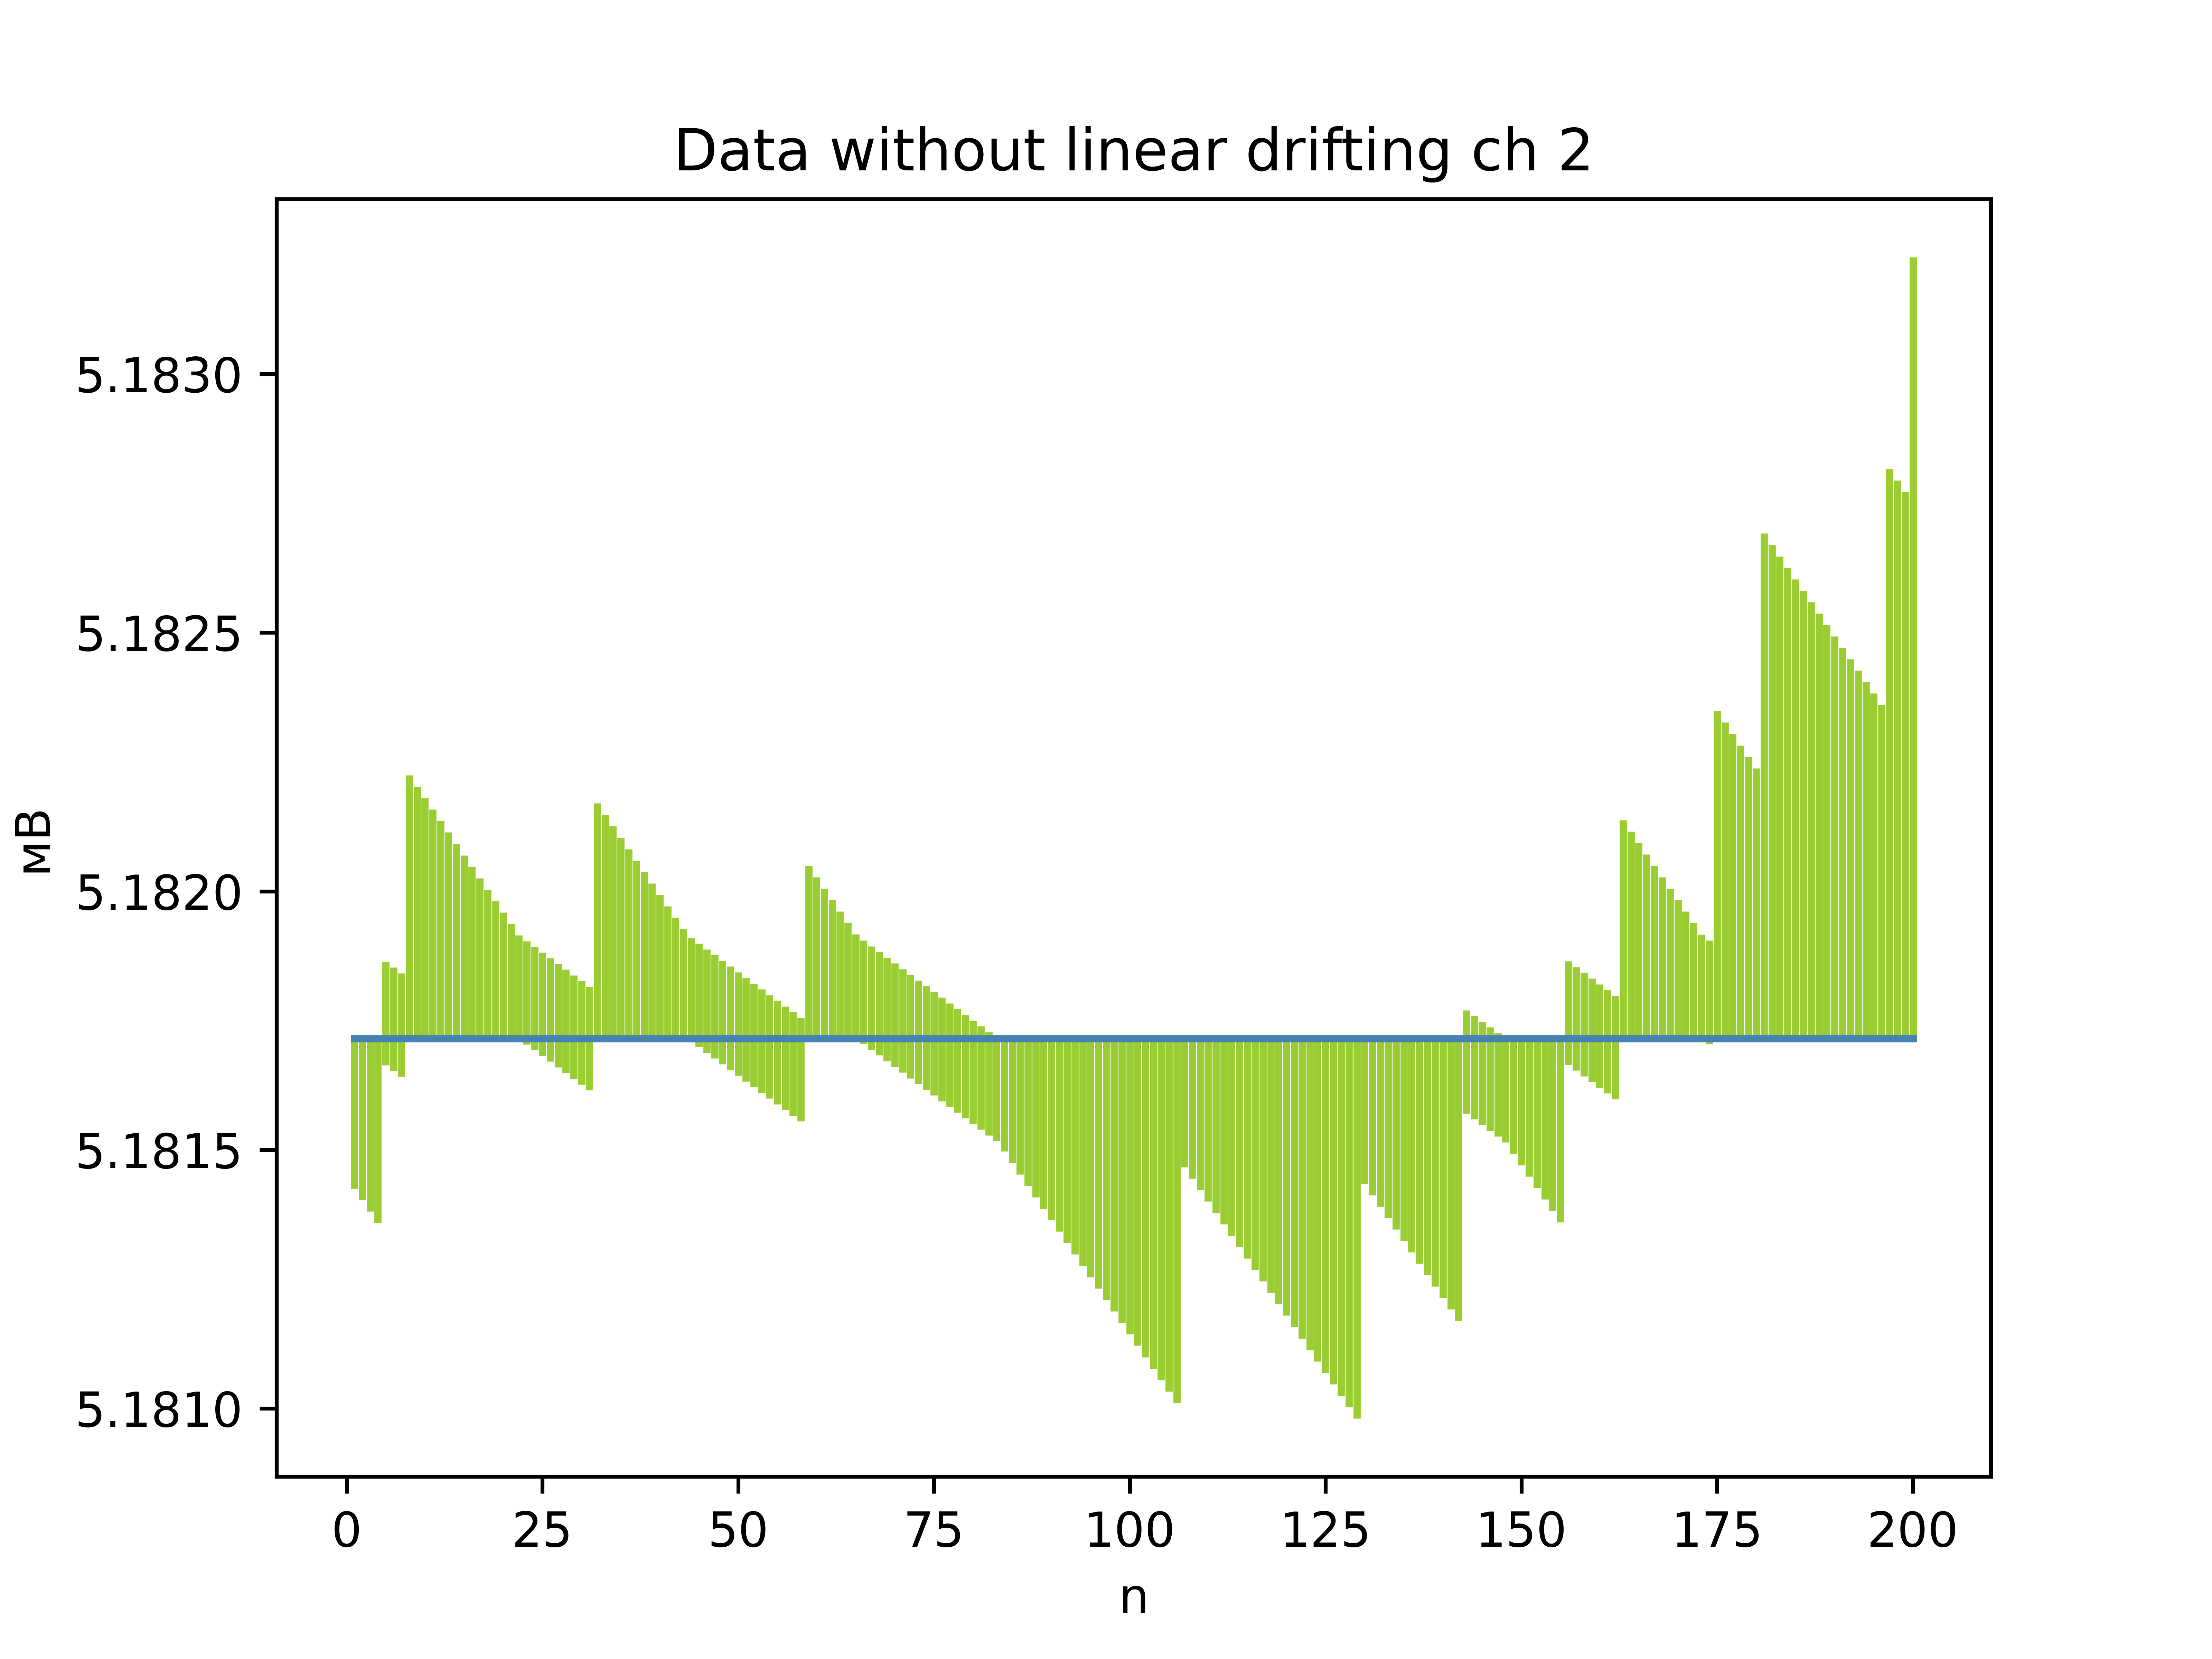
\includegraphics[scale=0.5]{resources/fixed_PR2.png}
	\end{tabular}
	\caption{Скорректированные модели данных} 
\end{figure}

\begin{figure}[H]
	\begin{tabular}{ccc}
		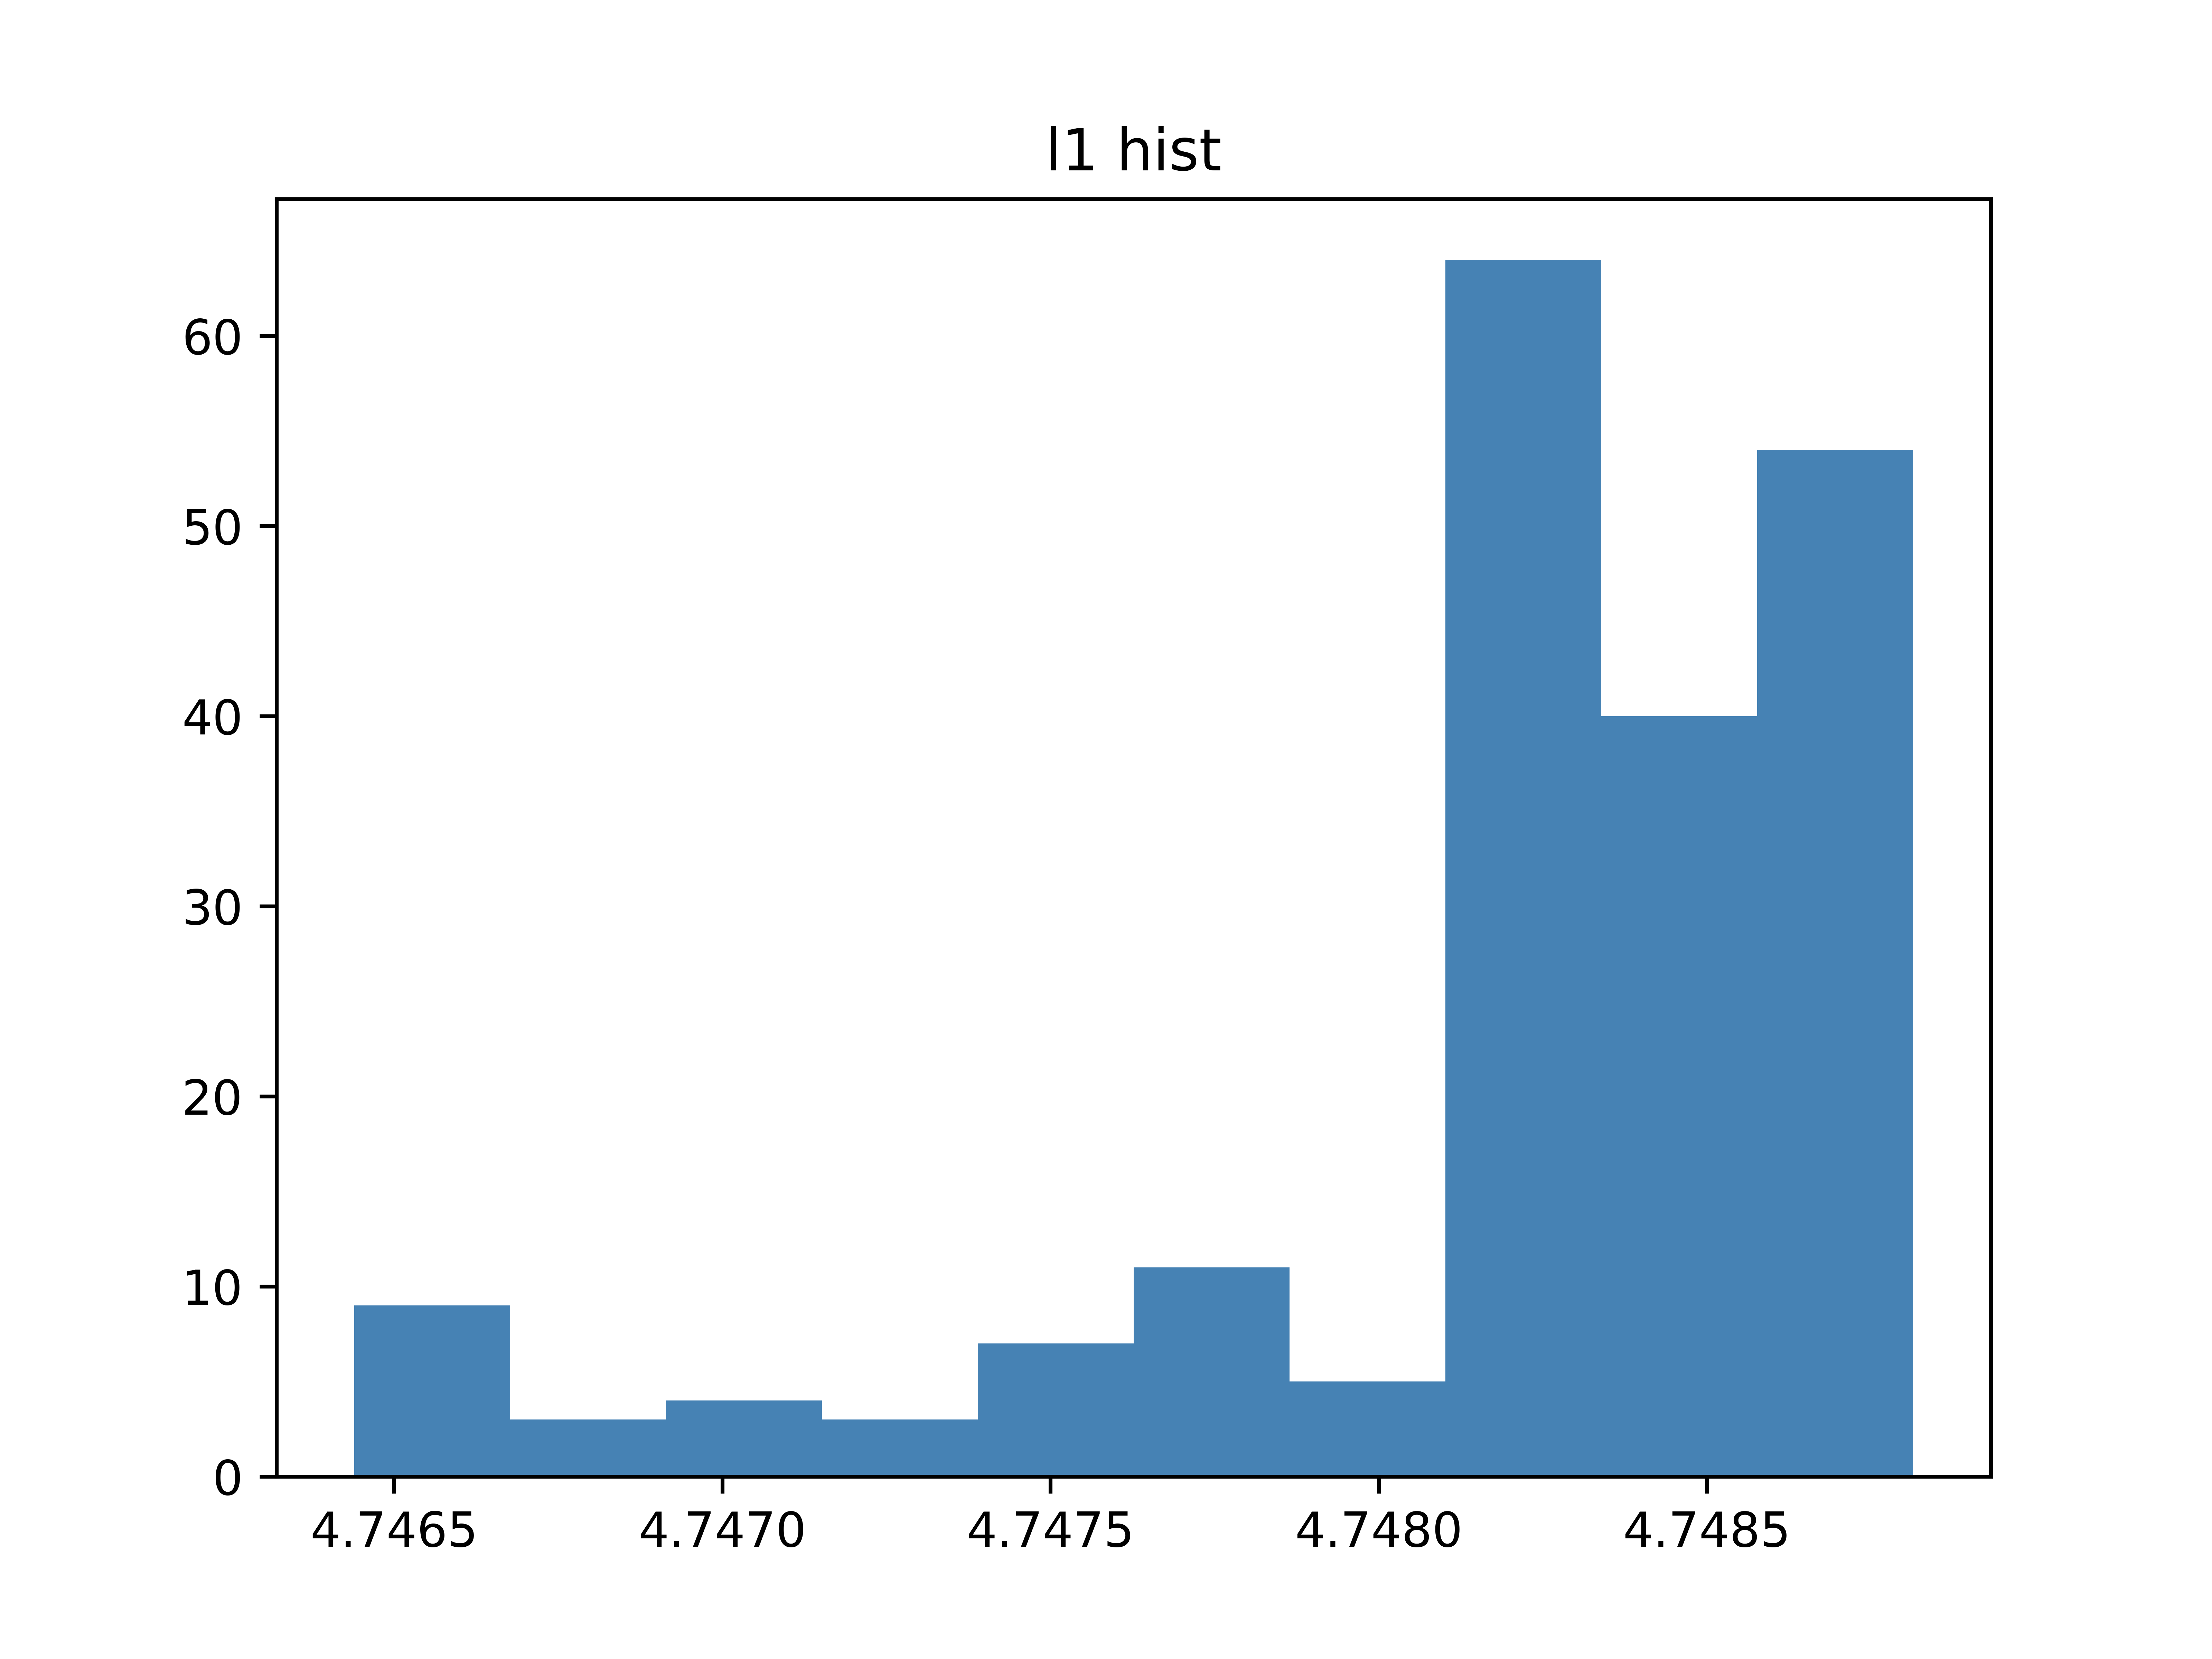
\includegraphics[scale=0.5]{resources/fhyst_PR1.png}
		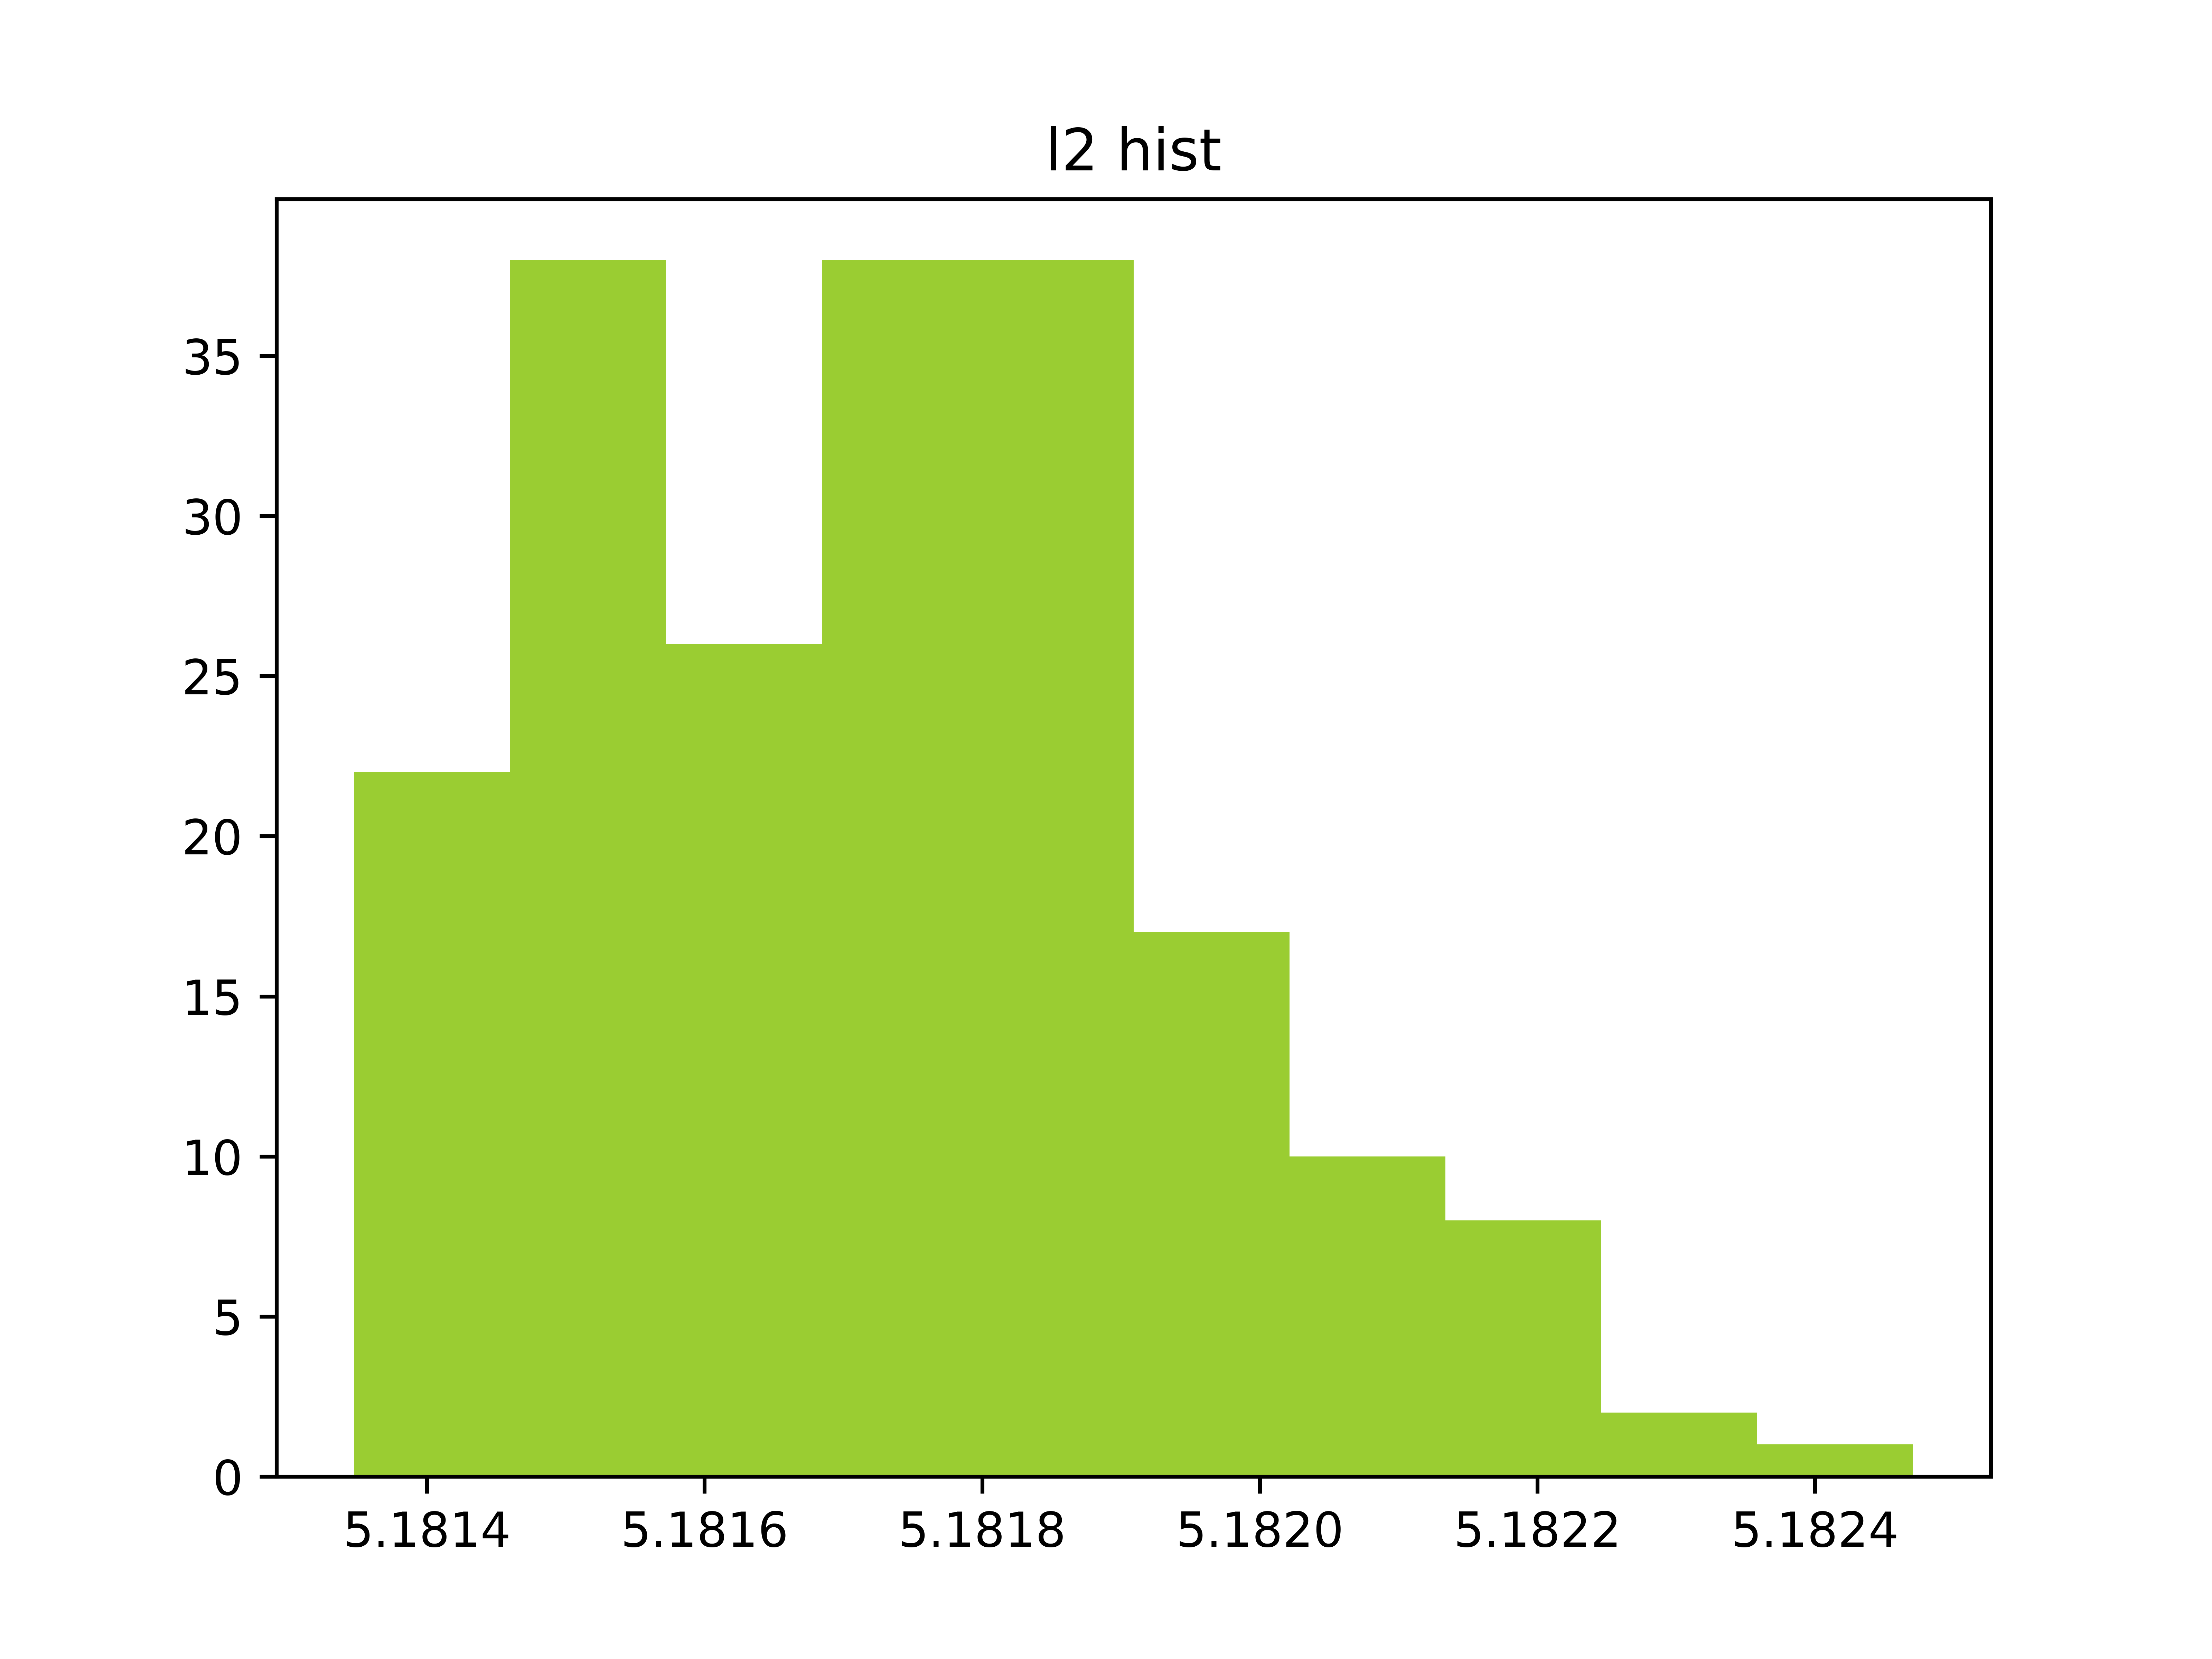
\includegraphics[scale=0.5]{resources/fhyst_PR2.png}
	\end{tabular} \label{pic:corrected}
	\caption{Гистограммы скорректированных данных} 
\end{figure}

\begin{figure}[H]
	\begin{center}
		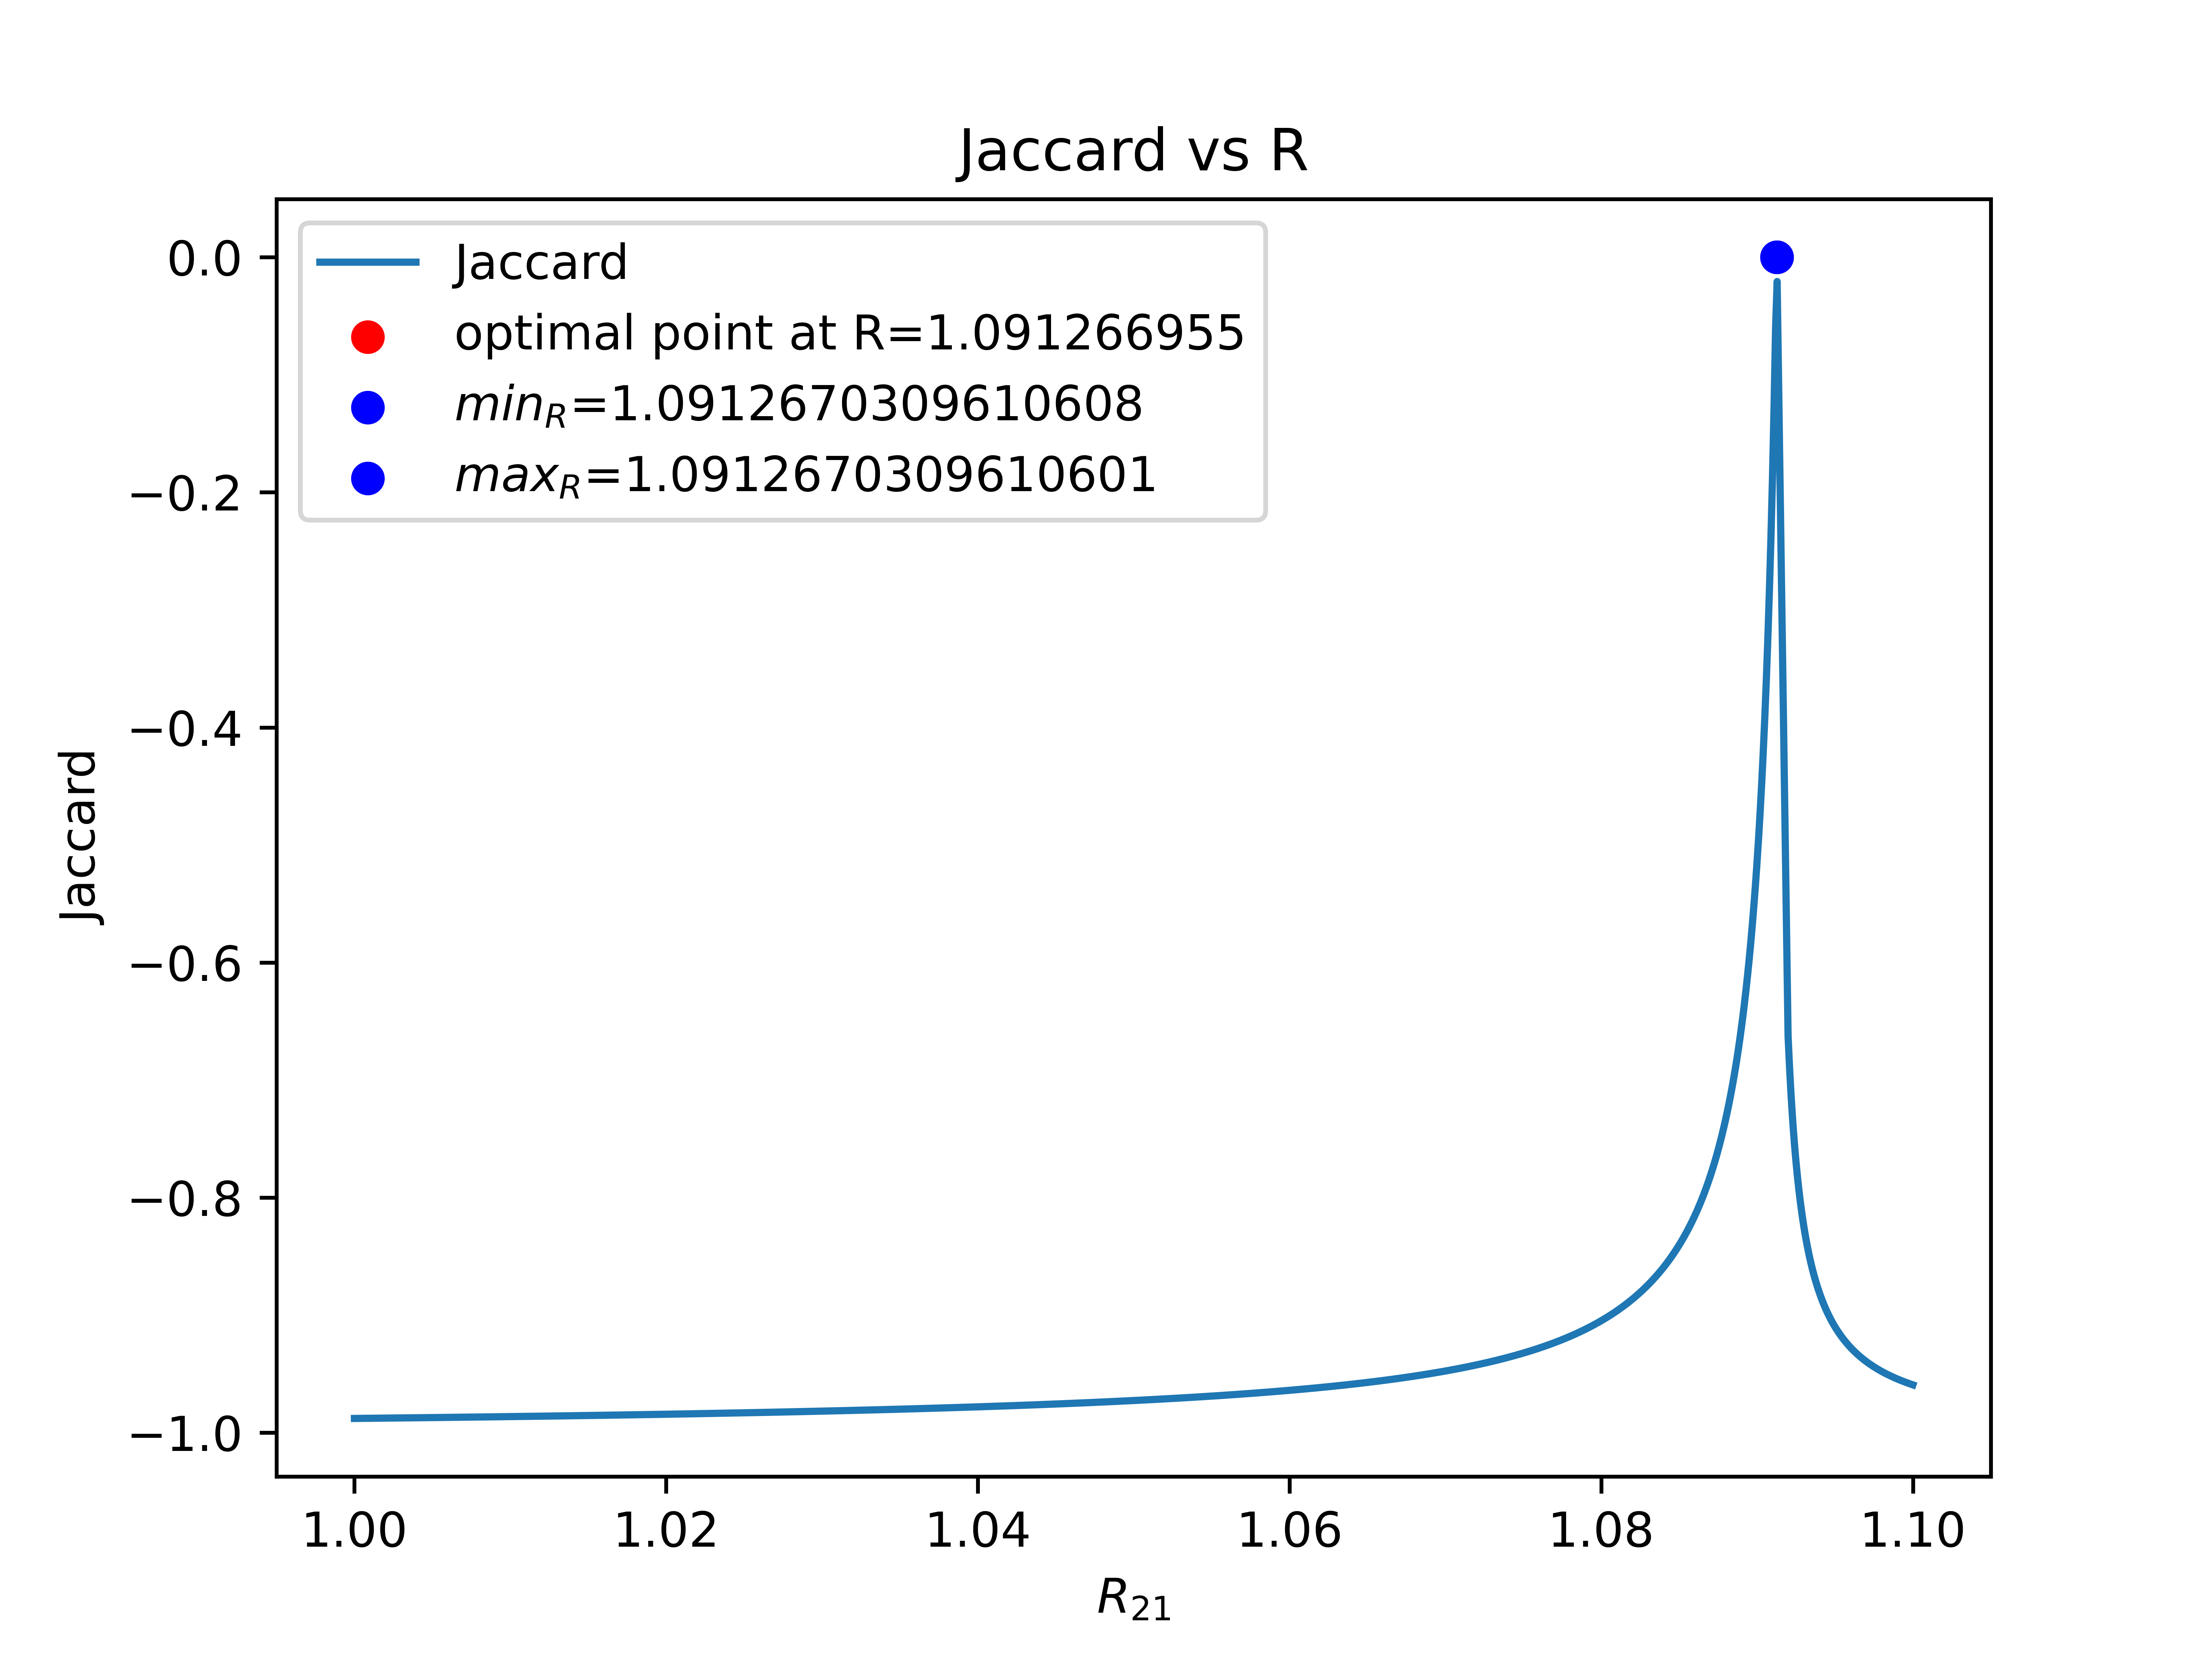
\includegraphics[scale=0.5]{resources/jakkar.png}
	\end{center} \label{pic:jaccar}
	\caption{Значение коэффициента Жаккара от калибровочного множителя от $R_{21}$} 
\end{figure}

\begin{figure}[H]
	\begin{center}
		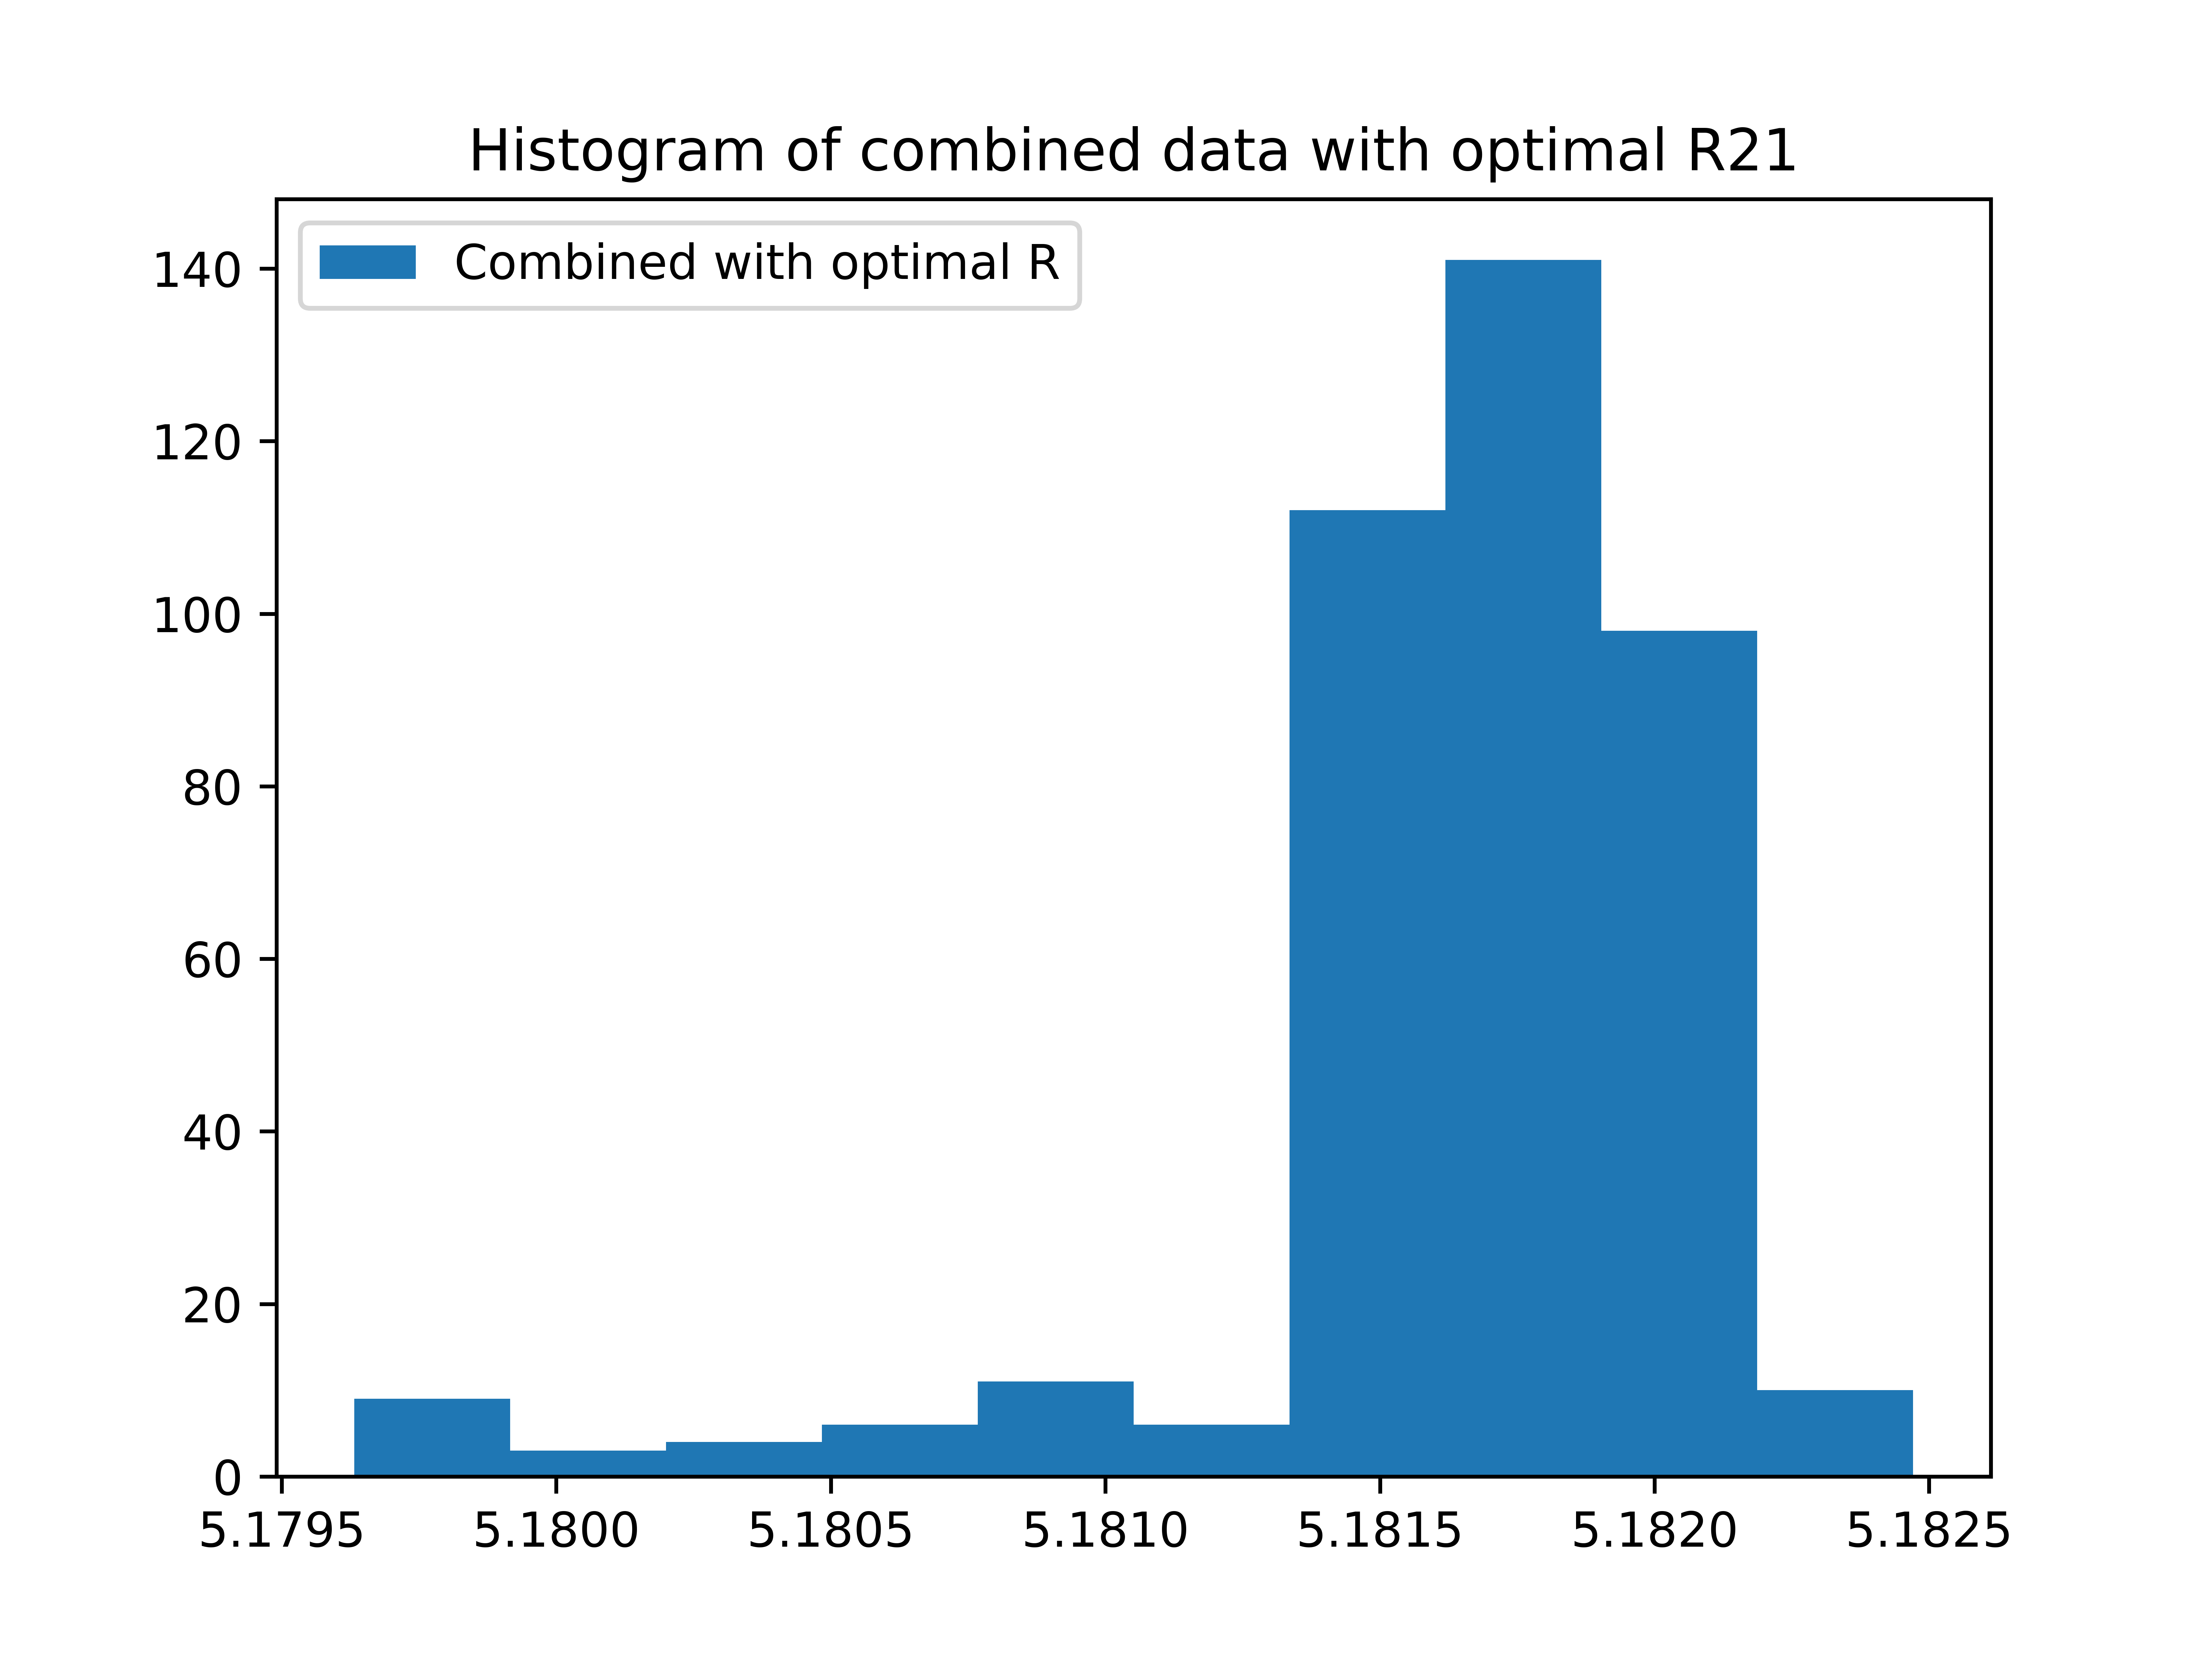
\includegraphics[scale=0.5]{resources/jakkar_combined_hist.png}
	\end{center} \label{pic:union}
	\caption{Гистограмма объединнённых данных при оптимальном значении $R_{21}$} 
\end{figure}

\newpage